\documentclass{article}
\usepackage[final]{neurips_2025}  % NEURIPS style (neurips_2025.sty is in paper_draft/)
% neurips_2025.sty defines the footer track name only under a track option; define the main-track text here
\makeatletter
\providecommand{\@trackname}{\@neuripsordinal\ Conference on Neural Information Processing Systems (NeurIPS \@neuripsyear).}
\makeatother
\usepackage[hidelinks]{hyperref}  % REQUIRED: clickable links
\usepackage{booktabs}  % REQUIRED: professional tables
\usepackage{graphicx}
\usepackage{amsmath,amssymb}
\usepackage[utf8]{inputenc}
\usepackage[T1]{fontenc}
\usepackage{enumitem}
\usepackage{multirow}
\usepackage{tabularx}
\usepackage{algorithm}
\usepackage[noend]{algpseudocode}
\usepackage{tikz}
\usetikzlibrary{positioning,arrows.meta,fit}

% Import command files
%%%%% MATH NOTATION MACROS %%%%%
% Standard math notation for academic papers
% Import with: %%%%% MATH NOTATION MACROS %%%%%
% Standard math notation for academic papers
% Import with: %%%%% MATH NOTATION MACROS %%%%%
% Standard math notation for academic papers
% Import with: \input{commands/math}

\usepackage{amsmath,amsfonts,bm}

%%%%%%%%%%%%%%%%%%%%%%%%%%%%%%%%%%%%%%%%%%%%%%%%%%%%%%%%%%%%%%%%%
% FIGURE AND SECTION REFERENCES
%%%%%%%%%%%%%%%%%%%%%%%%%%%%%%%%%%%%%%%%%%%%%%%%%%%%%%%%%%%%%%%%%

% Mark sections of captions for referring to divisions of figures
\newcommand{\figleft}{{\em (Left)}}
\newcommand{\figcenter}{{\em (Center)}}
\newcommand{\figright}{{\em (Right)}}
\newcommand{\figtop}{{\em (Top)}}
\newcommand{\figbottom}{{\em (Bottom)}}
\newcommand{\captiona}{{\em (a)}}
\newcommand{\captionb}{{\em (b)}}
\newcommand{\captionc}{{\em (c)}}
\newcommand{\captiond}{{\em (d)}}

% Figure references
\def\figref#1{figure~\ref{#1}}
\def\Figref#1{Figure~\ref{#1}}
\def\twofigref#1#2{figures \ref{#1} and \ref{#2}}
\def\quadfigref#1#2#3#4{figures \ref{#1}, \ref{#2}, \ref{#3} and \ref{#4}}

% Section references
\def\secref#1{section~\ref{#1}}
\def\Secref#1{Section~\ref{#1}}
\def\twosecrefs#1#2{sections \ref{#1} and \ref{#2}}
\def\secrefs#1#2#3{sections \ref{#1}, \ref{#2} and \ref{#3}}

% Equation references
\def\eqref#1{equation~\ref{#1}}
\def\Eqref#1{Equation~\ref{#1}}
\def\plaineqref#1{\ref{#1}}

% Algorithm references
\def\algref#1{algorithm~\ref{#1}}
\def\Algref#1{Algorithm~\ref{#1}}
\def\twoalgref#1#2{algorithms \ref{#1} and \ref{#2}}
\def\Twoalgref#1#2{Algorithms \ref{#1} and \ref{#2}}

% Table references
\def\tabref#1{table~\ref{#1}}
\def\Tabref#1{Table~\ref{#1}}

% Chapter references
\def\chapref#1{chapter~\ref{#1}}
\def\Chapref#1{Chapter~\ref{#1}}

%%%%%%%%%%%%%%%%%%%%%%%%%%%%%%%%%%%%%%%%%%%%%%%%%%%%%%%%%%%%%%%%%
% BASIC MATH DEFINITIONS
%%%%%%%%%%%%%%%%%%%%%%%%%%%%%%%%%%%%%%%%%%%%%%%%%%%%%%%%%%%%%%%%%

\def\ceil#1{\lceil #1 \rceil}
\def\floor#1{\lfloor #1 \rfloor}
\def\1{\bm{1}}
\def\eps{{\epsilon}}

% Common operators
\DeclareMathOperator*{\argmax}{arg\,max}
\DeclareMathOperator*{\argmin}{arg\,min}
\DeclareMathOperator{\sign}{sign}
\DeclareMathOperator{\Tr}{Tr}
\let\ab\allowbreak

%%%%%%%%%%%%%%%%%%%%%%%%%%%%%%%%%%%%%%%%%%%%%%%%%%%%%%%%%%%%%%%%%
% VECTORS (lowercase bold)
%%%%%%%%%%%%%%%%%%%%%%%%%%%%%%%%%%%%%%%%%%%%%%%%%%%%%%%%%%%%%%%%%

\def\vzero{{\bm{0}}}
\def\vone{{\bm{1}}}
\def\vmu{{\bm{\mu}}}
\def\vtheta{{\bm{\theta}}}
\def\va{{\bm{a}}}
\def\vb{{\bm{b}}}
\def\vc{{\bm{c}}}
\def\vd{{\bm{d}}}
\def\ve{{\bm{e}}}
\def\vf{{\bm{f}}}
\def\vg{{\bm{g}}}
\def\vh{{\bm{h}}}
\def\vi{{\bm{i}}}
\def\vj{{\bm{j}}}
\def\vk{{\bm{k}}}
\def\vl{{\bm{l}}}
\def\vm{{\bm{m}}}
\def\vn{{\bm{n}}}
\def\vo{{\bm{o}}}
\def\vp{{\bm{p}}}
\def\vq{{\bm{q}}}
\def\vr{{\bm{r}}}
\def\vs{{\bm{s}}}
\def\vt{{\bm{t}}}
\def\vu{{\bm{u}}}
\def\vv{{\bm{v}}}
\def\vw{{\bm{w}}}
\def\vx{{\bm{x}}}
\def\vy{{\bm{y}}}
\def\vz{{\bm{z}}}

%%%%%%%%%%%%%%%%%%%%%%%%%%%%%%%%%%%%%%%%%%%%%%%%%%%%%%%%%%%%%%%%%
% MATRICES (uppercase bold)
%%%%%%%%%%%%%%%%%%%%%%%%%%%%%%%%%%%%%%%%%%%%%%%%%%%%%%%%%%%%%%%%%

\def\mA{{\bm{A}}}
\def\mB{{\bm{B}}}
\def\mC{{\bm{C}}}
\def\mD{{\bm{D}}}
\def\mE{{\bm{E}}}
\def\mF{{\bm{F}}}
\def\mG{{\bm{G}}}
\def\mH{{\bm{H}}}
\def\mI{{\bm{I}}}
\def\mJ{{\bm{J}}}
\def\mK{{\bm{K}}}
\def\mL{{\bm{L}}}
\def\mM{{\bm{M}}}
\def\mN{{\bm{N}}}
\def\mO{{\bm{O}}}
\def\mP{{\bm{P}}}
\def\mQ{{\bm{Q}}}
\def\mR{{\bm{R}}}
\def\mS{{\bm{S}}}
\def\mT{{\bm{T}}}
\def\mU{{\bm{U}}}
\def\mV{{\bm{V}}}
\def\mW{{\bm{W}}}
\def\mX{{\bm{X}}}
\def\mY{{\bm{Y}}}
\def\mZ{{\bm{Z}}}
\def\mBeta{{\bm{\beta}}}
\def\mPhi{{\bm{\Phi}}}
\def\mLambda{{\bm{\Lambda}}}
\def\mSigma{{\bm{\Sigma}}}

%%%%%%%%%%%%%%%%%%%%%%%%%%%%%%%%%%%%%%%%%%%%%%%%%%%%%%%%%%%%%%%%%
% CALLIGRAPHIC (mathcal)
%%%%%%%%%%%%%%%%%%%%%%%%%%%%%%%%%%%%%%%%%%%%%%%%%%%%%%%%%%%%%%%%%

\def\gA{{\mathcal{A}}}
\def\gB{{\mathcal{B}}}
\def\gC{{\mathcal{C}}}
\def\gD{{\mathcal{D}}}
\def\gE{{\mathcal{E}}}
\def\gF{{\mathcal{F}}}
\def\gG{{\mathcal{G}}}
\def\gH{{\mathcal{H}}}
\def\gI{{\mathcal{I}}}
\def\gJ{{\mathcal{J}}}
\def\gK{{\mathcal{K}}}
\def\gL{{\mathcal{L}}}
\def\gM{{\mathcal{M}}}
\def\gN{{\mathcal{N}}}
\def\gO{{\mathcal{O}}}
\def\gP{{\mathcal{P}}}
\def\gQ{{\mathcal{Q}}}
\def\gR{{\mathcal{R}}}
\def\gS{{\mathcal{S}}}
\def\gT{{\mathcal{T}}}
\def\gU{{\mathcal{U}}}
\def\gV{{\mathcal{V}}}
\def\gW{{\mathcal{W}}}
\def\gX{{\mathcal{X}}}
\def\gY{{\mathcal{Y}}}
\def\gZ{{\mathcal{Z}}}

%%%%%%%%%%%%%%%%%%%%%%%%%%%%%%%%%%%%%%%%%%%%%%%%%%%%%%%%%%%%%%%%%
% SETS (blackboard bold)
%%%%%%%%%%%%%%%%%%%%%%%%%%%%%%%%%%%%%%%%%%%%%%%%%%%%%%%%%%%%%%%%%

\def\sA{{\mathbb{A}}}
\def\sB{{\mathbb{B}}}
\def\sC{{\mathbb{C}}}
\def\sD{{\mathbb{D}}}
\def\sF{{\mathbb{F}}}
\def\sG{{\mathbb{G}}}
\def\sH{{\mathbb{H}}}
\def\sI{{\mathbb{I}}}
\def\sJ{{\mathbb{J}}}
\def\sK{{\mathbb{K}}}
\def\sL{{\mathbb{L}}}
\def\sM{{\mathbb{M}}}
\def\sN{{\mathbb{N}}}
\def\sO{{\mathbb{O}}}
\def\sP{{\mathbb{P}}}
\def\sQ{{\mathbb{Q}}}
\def\sR{{\mathbb{R}}}
\def\sS{{\mathbb{S}}}
\def\sT{{\mathbb{T}}}
\def\sU{{\mathbb{U}}}
\def\sV{{\mathbb{V}}}
\def\sW{{\mathbb{W}}}
\def\sX{{\mathbb{X}}}
\def\sY{{\mathbb{Y}}}
\def\sZ{{\mathbb{Z}}}

%%%%%%%%%%%%%%%%%%%%%%%%%%%%%%%%%%%%%%%%%%%%%%%%%%%%%%%%%%%%%%%%%
% COMMON MATH SHORTCUTS
%%%%%%%%%%%%%%%%%%%%%%%%%%%%%%%%%%%%%%%%%%%%%%%%%%%%%%%%%%%%%%%%%

% Expectation and variance
\newcommand{\E}{\mathbb{E}}
\newcommand{\Var}{\mathrm{Var}}
\newcommand{\Cov}{\mathrm{Cov}}
\newcommand{\R}{\mathbb{R}}

% Datasets
\newcommand{\train}{\mathcal{D}}
\newcommand{\valid}{\mathcal{D_{\mathrm{valid}}}}
\newcommand{\test}{\mathcal{D_{\mathrm{test}}}}

% Distributions
\newcommand{\laplace}{\mathrm{Laplace}}
\newcommand{\Uniform}{\mathrm{Unif}}
\newcommand{\Normal}{\mathrm{Normal}}
\newcommand{\Categorical}{\mathrm{Categorical}}

% Common functions
\newcommand{\softmax}{\mathrm{softmax}}
\newcommand{\sigmoid}{\sigma}
\newcommand{\KL}{D_{\mathrm{KL}}}

% Norms
\newcommand{\normlzero}{L^0}
\newcommand{\normlone}{L^1}
\newcommand{\normltwo}{L^2}
\newcommand{\normlp}{L^p}
\newcommand{\normmax}{L^\infty}

%%%%%%%%%%%%%%%%%%%%%%%%%%%%%%%%%%%%%%%%%%%%%%%%%%%%%%%%%%%%%%%%%
% DEFINITIONS AND HIGHLIGHTING
%%%%%%%%%%%%%%%%%%%%%%%%%%%%%%%%%%%%%%%%%%%%%%%%%%%%%%%%%%%%%%%%%

% Highlight a newly defined term
\newcommand{\newterm}[1]{{\bf #1}}
\newcommand{\defn}[1]{\textbf{#1}}
\newcommand{\defeq}{\mathrel{\stackrel{\textnormal{\tiny def}}{=}}}


\usepackage{amsmath,amsfonts,bm}

%%%%%%%%%%%%%%%%%%%%%%%%%%%%%%%%%%%%%%%%%%%%%%%%%%%%%%%%%%%%%%%%%
% FIGURE AND SECTION REFERENCES
%%%%%%%%%%%%%%%%%%%%%%%%%%%%%%%%%%%%%%%%%%%%%%%%%%%%%%%%%%%%%%%%%

% Mark sections of captions for referring to divisions of figures
\newcommand{\figleft}{{\em (Left)}}
\newcommand{\figcenter}{{\em (Center)}}
\newcommand{\figright}{{\em (Right)}}
\newcommand{\figtop}{{\em (Top)}}
\newcommand{\figbottom}{{\em (Bottom)}}
\newcommand{\captiona}{{\em (a)}}
\newcommand{\captionb}{{\em (b)}}
\newcommand{\captionc}{{\em (c)}}
\newcommand{\captiond}{{\em (d)}}

% Figure references
\def\figref#1{figure~\ref{#1}}
\def\Figref#1{Figure~\ref{#1}}
\def\twofigref#1#2{figures \ref{#1} and \ref{#2}}
\def\quadfigref#1#2#3#4{figures \ref{#1}, \ref{#2}, \ref{#3} and \ref{#4}}

% Section references
\def\secref#1{section~\ref{#1}}
\def\Secref#1{Section~\ref{#1}}
\def\twosecrefs#1#2{sections \ref{#1} and \ref{#2}}
\def\secrefs#1#2#3{sections \ref{#1}, \ref{#2} and \ref{#3}}

% Equation references
\def\eqref#1{equation~\ref{#1}}
\def\Eqref#1{Equation~\ref{#1}}
\def\plaineqref#1{\ref{#1}}

% Algorithm references
\def\algref#1{algorithm~\ref{#1}}
\def\Algref#1{Algorithm~\ref{#1}}
\def\twoalgref#1#2{algorithms \ref{#1} and \ref{#2}}
\def\Twoalgref#1#2{Algorithms \ref{#1} and \ref{#2}}

% Table references
\def\tabref#1{table~\ref{#1}}
\def\Tabref#1{Table~\ref{#1}}

% Chapter references
\def\chapref#1{chapter~\ref{#1}}
\def\Chapref#1{Chapter~\ref{#1}}

%%%%%%%%%%%%%%%%%%%%%%%%%%%%%%%%%%%%%%%%%%%%%%%%%%%%%%%%%%%%%%%%%
% BASIC MATH DEFINITIONS
%%%%%%%%%%%%%%%%%%%%%%%%%%%%%%%%%%%%%%%%%%%%%%%%%%%%%%%%%%%%%%%%%

\def\ceil#1{\lceil #1 \rceil}
\def\floor#1{\lfloor #1 \rfloor}
\def\1{\bm{1}}
\def\eps{{\epsilon}}

% Common operators
\DeclareMathOperator*{\argmax}{arg\,max}
\DeclareMathOperator*{\argmin}{arg\,min}
\DeclareMathOperator{\sign}{sign}
\DeclareMathOperator{\Tr}{Tr}
\let\ab\allowbreak

%%%%%%%%%%%%%%%%%%%%%%%%%%%%%%%%%%%%%%%%%%%%%%%%%%%%%%%%%%%%%%%%%
% VECTORS (lowercase bold)
%%%%%%%%%%%%%%%%%%%%%%%%%%%%%%%%%%%%%%%%%%%%%%%%%%%%%%%%%%%%%%%%%

\def\vzero{{\bm{0}}}
\def\vone{{\bm{1}}}
\def\vmu{{\bm{\mu}}}
\def\vtheta{{\bm{\theta}}}
\def\va{{\bm{a}}}
\def\vb{{\bm{b}}}
\def\vc{{\bm{c}}}
\def\vd{{\bm{d}}}
\def\ve{{\bm{e}}}
\def\vf{{\bm{f}}}
\def\vg{{\bm{g}}}
\def\vh{{\bm{h}}}
\def\vi{{\bm{i}}}
\def\vj{{\bm{j}}}
\def\vk{{\bm{k}}}
\def\vl{{\bm{l}}}
\def\vm{{\bm{m}}}
\def\vn{{\bm{n}}}
\def\vo{{\bm{o}}}
\def\vp{{\bm{p}}}
\def\vq{{\bm{q}}}
\def\vr{{\bm{r}}}
\def\vs{{\bm{s}}}
\def\vt{{\bm{t}}}
\def\vu{{\bm{u}}}
\def\vv{{\bm{v}}}
\def\vw{{\bm{w}}}
\def\vx{{\bm{x}}}
\def\vy{{\bm{y}}}
\def\vz{{\bm{z}}}

%%%%%%%%%%%%%%%%%%%%%%%%%%%%%%%%%%%%%%%%%%%%%%%%%%%%%%%%%%%%%%%%%
% MATRICES (uppercase bold)
%%%%%%%%%%%%%%%%%%%%%%%%%%%%%%%%%%%%%%%%%%%%%%%%%%%%%%%%%%%%%%%%%

\def\mA{{\bm{A}}}
\def\mB{{\bm{B}}}
\def\mC{{\bm{C}}}
\def\mD{{\bm{D}}}
\def\mE{{\bm{E}}}
\def\mF{{\bm{F}}}
\def\mG{{\bm{G}}}
\def\mH{{\bm{H}}}
\def\mI{{\bm{I}}}
\def\mJ{{\bm{J}}}
\def\mK{{\bm{K}}}
\def\mL{{\bm{L}}}
\def\mM{{\bm{M}}}
\def\mN{{\bm{N}}}
\def\mO{{\bm{O}}}
\def\mP{{\bm{P}}}
\def\mQ{{\bm{Q}}}
\def\mR{{\bm{R}}}
\def\mS{{\bm{S}}}
\def\mT{{\bm{T}}}
\def\mU{{\bm{U}}}
\def\mV{{\bm{V}}}
\def\mW{{\bm{W}}}
\def\mX{{\bm{X}}}
\def\mY{{\bm{Y}}}
\def\mZ{{\bm{Z}}}
\def\mBeta{{\bm{\beta}}}
\def\mPhi{{\bm{\Phi}}}
\def\mLambda{{\bm{\Lambda}}}
\def\mSigma{{\bm{\Sigma}}}

%%%%%%%%%%%%%%%%%%%%%%%%%%%%%%%%%%%%%%%%%%%%%%%%%%%%%%%%%%%%%%%%%
% CALLIGRAPHIC (mathcal)
%%%%%%%%%%%%%%%%%%%%%%%%%%%%%%%%%%%%%%%%%%%%%%%%%%%%%%%%%%%%%%%%%

\def\gA{{\mathcal{A}}}
\def\gB{{\mathcal{B}}}
\def\gC{{\mathcal{C}}}
\def\gD{{\mathcal{D}}}
\def\gE{{\mathcal{E}}}
\def\gF{{\mathcal{F}}}
\def\gG{{\mathcal{G}}}
\def\gH{{\mathcal{H}}}
\def\gI{{\mathcal{I}}}
\def\gJ{{\mathcal{J}}}
\def\gK{{\mathcal{K}}}
\def\gL{{\mathcal{L}}}
\def\gM{{\mathcal{M}}}
\def\gN{{\mathcal{N}}}
\def\gO{{\mathcal{O}}}
\def\gP{{\mathcal{P}}}
\def\gQ{{\mathcal{Q}}}
\def\gR{{\mathcal{R}}}
\def\gS{{\mathcal{S}}}
\def\gT{{\mathcal{T}}}
\def\gU{{\mathcal{U}}}
\def\gV{{\mathcal{V}}}
\def\gW{{\mathcal{W}}}
\def\gX{{\mathcal{X}}}
\def\gY{{\mathcal{Y}}}
\def\gZ{{\mathcal{Z}}}

%%%%%%%%%%%%%%%%%%%%%%%%%%%%%%%%%%%%%%%%%%%%%%%%%%%%%%%%%%%%%%%%%
% SETS (blackboard bold)
%%%%%%%%%%%%%%%%%%%%%%%%%%%%%%%%%%%%%%%%%%%%%%%%%%%%%%%%%%%%%%%%%

\def\sA{{\mathbb{A}}}
\def\sB{{\mathbb{B}}}
\def\sC{{\mathbb{C}}}
\def\sD{{\mathbb{D}}}
\def\sF{{\mathbb{F}}}
\def\sG{{\mathbb{G}}}
\def\sH{{\mathbb{H}}}
\def\sI{{\mathbb{I}}}
\def\sJ{{\mathbb{J}}}
\def\sK{{\mathbb{K}}}
\def\sL{{\mathbb{L}}}
\def\sM{{\mathbb{M}}}
\def\sN{{\mathbb{N}}}
\def\sO{{\mathbb{O}}}
\def\sP{{\mathbb{P}}}
\def\sQ{{\mathbb{Q}}}
\def\sR{{\mathbb{R}}}
\def\sS{{\mathbb{S}}}
\def\sT{{\mathbb{T}}}
\def\sU{{\mathbb{U}}}
\def\sV{{\mathbb{V}}}
\def\sW{{\mathbb{W}}}
\def\sX{{\mathbb{X}}}
\def\sY{{\mathbb{Y}}}
\def\sZ{{\mathbb{Z}}}

%%%%%%%%%%%%%%%%%%%%%%%%%%%%%%%%%%%%%%%%%%%%%%%%%%%%%%%%%%%%%%%%%
% COMMON MATH SHORTCUTS
%%%%%%%%%%%%%%%%%%%%%%%%%%%%%%%%%%%%%%%%%%%%%%%%%%%%%%%%%%%%%%%%%

% Expectation and variance
\newcommand{\E}{\mathbb{E}}
\newcommand{\Var}{\mathrm{Var}}
\newcommand{\Cov}{\mathrm{Cov}}
\newcommand{\R}{\mathbb{R}}

% Datasets
\newcommand{\train}{\mathcal{D}}
\newcommand{\valid}{\mathcal{D_{\mathrm{valid}}}}
\newcommand{\test}{\mathcal{D_{\mathrm{test}}}}

% Distributions
\newcommand{\laplace}{\mathrm{Laplace}}
\newcommand{\Uniform}{\mathrm{Unif}}
\newcommand{\Normal}{\mathrm{Normal}}
\newcommand{\Categorical}{\mathrm{Categorical}}

% Common functions
\newcommand{\softmax}{\mathrm{softmax}}
\newcommand{\sigmoid}{\sigma}
\newcommand{\KL}{D_{\mathrm{KL}}}

% Norms
\newcommand{\normlzero}{L^0}
\newcommand{\normlone}{L^1}
\newcommand{\normltwo}{L^2}
\newcommand{\normlp}{L^p}
\newcommand{\normmax}{L^\infty}

%%%%%%%%%%%%%%%%%%%%%%%%%%%%%%%%%%%%%%%%%%%%%%%%%%%%%%%%%%%%%%%%%
% DEFINITIONS AND HIGHLIGHTING
%%%%%%%%%%%%%%%%%%%%%%%%%%%%%%%%%%%%%%%%%%%%%%%%%%%%%%%%%%%%%%%%%

% Highlight a newly defined term
\newcommand{\newterm}[1]{{\bf #1}}
\newcommand{\defn}[1]{\textbf{#1}}
\newcommand{\defeq}{\mathrel{\stackrel{\textnormal{\tiny def}}{=}}}


\usepackage{amsmath,amsfonts,bm}

%%%%%%%%%%%%%%%%%%%%%%%%%%%%%%%%%%%%%%%%%%%%%%%%%%%%%%%%%%%%%%%%%
% FIGURE AND SECTION REFERENCES
%%%%%%%%%%%%%%%%%%%%%%%%%%%%%%%%%%%%%%%%%%%%%%%%%%%%%%%%%%%%%%%%%

% Mark sections of captions for referring to divisions of figures
\newcommand{\figleft}{{\em (Left)}}
\newcommand{\figcenter}{{\em (Center)}}
\newcommand{\figright}{{\em (Right)}}
\newcommand{\figtop}{{\em (Top)}}
\newcommand{\figbottom}{{\em (Bottom)}}
\newcommand{\captiona}{{\em (a)}}
\newcommand{\captionb}{{\em (b)}}
\newcommand{\captionc}{{\em (c)}}
\newcommand{\captiond}{{\em (d)}}

% Figure references
\def\figref#1{figure~\ref{#1}}
\def\Figref#1{Figure~\ref{#1}}
\def\twofigref#1#2{figures \ref{#1} and \ref{#2}}
\def\quadfigref#1#2#3#4{figures \ref{#1}, \ref{#2}, \ref{#3} and \ref{#4}}

% Section references
\def\secref#1{section~\ref{#1}}
\def\Secref#1{Section~\ref{#1}}
\def\twosecrefs#1#2{sections \ref{#1} and \ref{#2}}
\def\secrefs#1#2#3{sections \ref{#1}, \ref{#2} and \ref{#3}}

% Equation references
\def\eqref#1{equation~\ref{#1}}
\def\Eqref#1{Equation~\ref{#1}}
\def\plaineqref#1{\ref{#1}}

% Algorithm references
\def\algref#1{algorithm~\ref{#1}}
\def\Algref#1{Algorithm~\ref{#1}}
\def\twoalgref#1#2{algorithms \ref{#1} and \ref{#2}}
\def\Twoalgref#1#2{Algorithms \ref{#1} and \ref{#2}}

% Table references
\def\tabref#1{table~\ref{#1}}
\def\Tabref#1{Table~\ref{#1}}

% Chapter references
\def\chapref#1{chapter~\ref{#1}}
\def\Chapref#1{Chapter~\ref{#1}}

%%%%%%%%%%%%%%%%%%%%%%%%%%%%%%%%%%%%%%%%%%%%%%%%%%%%%%%%%%%%%%%%%
% BASIC MATH DEFINITIONS
%%%%%%%%%%%%%%%%%%%%%%%%%%%%%%%%%%%%%%%%%%%%%%%%%%%%%%%%%%%%%%%%%

\def\ceil#1{\lceil #1 \rceil}
\def\floor#1{\lfloor #1 \rfloor}
\def\1{\bm{1}}
\def\eps{{\epsilon}}

% Common operators
\DeclareMathOperator*{\argmax}{arg\,max}
\DeclareMathOperator*{\argmin}{arg\,min}
\DeclareMathOperator{\sign}{sign}
\DeclareMathOperator{\Tr}{Tr}
\let\ab\allowbreak

%%%%%%%%%%%%%%%%%%%%%%%%%%%%%%%%%%%%%%%%%%%%%%%%%%%%%%%%%%%%%%%%%
% VECTORS (lowercase bold)
%%%%%%%%%%%%%%%%%%%%%%%%%%%%%%%%%%%%%%%%%%%%%%%%%%%%%%%%%%%%%%%%%

\def\vzero{{\bm{0}}}
\def\vone{{\bm{1}}}
\def\vmu{{\bm{\mu}}}
\def\vtheta{{\bm{\theta}}}
\def\va{{\bm{a}}}
\def\vb{{\bm{b}}}
\def\vc{{\bm{c}}}
\def\vd{{\bm{d}}}
\def\ve{{\bm{e}}}
\def\vf{{\bm{f}}}
\def\vg{{\bm{g}}}
\def\vh{{\bm{h}}}
\def\vi{{\bm{i}}}
\def\vj{{\bm{j}}}
\def\vk{{\bm{k}}}
\def\vl{{\bm{l}}}
\def\vm{{\bm{m}}}
\def\vn{{\bm{n}}}
\def\vo{{\bm{o}}}
\def\vp{{\bm{p}}}
\def\vq{{\bm{q}}}
\def\vr{{\bm{r}}}
\def\vs{{\bm{s}}}
\def\vt{{\bm{t}}}
\def\vu{{\bm{u}}}
\def\vv{{\bm{v}}}
\def\vw{{\bm{w}}}
\def\vx{{\bm{x}}}
\def\vy{{\bm{y}}}
\def\vz{{\bm{z}}}

%%%%%%%%%%%%%%%%%%%%%%%%%%%%%%%%%%%%%%%%%%%%%%%%%%%%%%%%%%%%%%%%%
% MATRICES (uppercase bold)
%%%%%%%%%%%%%%%%%%%%%%%%%%%%%%%%%%%%%%%%%%%%%%%%%%%%%%%%%%%%%%%%%

\def\mA{{\bm{A}}}
\def\mB{{\bm{B}}}
\def\mC{{\bm{C}}}
\def\mD{{\bm{D}}}
\def\mE{{\bm{E}}}
\def\mF{{\bm{F}}}
\def\mG{{\bm{G}}}
\def\mH{{\bm{H}}}
\def\mI{{\bm{I}}}
\def\mJ{{\bm{J}}}
\def\mK{{\bm{K}}}
\def\mL{{\bm{L}}}
\def\mM{{\bm{M}}}
\def\mN{{\bm{N}}}
\def\mO{{\bm{O}}}
\def\mP{{\bm{P}}}
\def\mQ{{\bm{Q}}}
\def\mR{{\bm{R}}}
\def\mS{{\bm{S}}}
\def\mT{{\bm{T}}}
\def\mU{{\bm{U}}}
\def\mV{{\bm{V}}}
\def\mW{{\bm{W}}}
\def\mX{{\bm{X}}}
\def\mY{{\bm{Y}}}
\def\mZ{{\bm{Z}}}
\def\mBeta{{\bm{\beta}}}
\def\mPhi{{\bm{\Phi}}}
\def\mLambda{{\bm{\Lambda}}}
\def\mSigma{{\bm{\Sigma}}}

%%%%%%%%%%%%%%%%%%%%%%%%%%%%%%%%%%%%%%%%%%%%%%%%%%%%%%%%%%%%%%%%%
% CALLIGRAPHIC (mathcal)
%%%%%%%%%%%%%%%%%%%%%%%%%%%%%%%%%%%%%%%%%%%%%%%%%%%%%%%%%%%%%%%%%

\def\gA{{\mathcal{A}}}
\def\gB{{\mathcal{B}}}
\def\gC{{\mathcal{C}}}
\def\gD{{\mathcal{D}}}
\def\gE{{\mathcal{E}}}
\def\gF{{\mathcal{F}}}
\def\gG{{\mathcal{G}}}
\def\gH{{\mathcal{H}}}
\def\gI{{\mathcal{I}}}
\def\gJ{{\mathcal{J}}}
\def\gK{{\mathcal{K}}}
\def\gL{{\mathcal{L}}}
\def\gM{{\mathcal{M}}}
\def\gN{{\mathcal{N}}}
\def\gO{{\mathcal{O}}}
\def\gP{{\mathcal{P}}}
\def\gQ{{\mathcal{Q}}}
\def\gR{{\mathcal{R}}}
\def\gS{{\mathcal{S}}}
\def\gT{{\mathcal{T}}}
\def\gU{{\mathcal{U}}}
\def\gV{{\mathcal{V}}}
\def\gW{{\mathcal{W}}}
\def\gX{{\mathcal{X}}}
\def\gY{{\mathcal{Y}}}
\def\gZ{{\mathcal{Z}}}

%%%%%%%%%%%%%%%%%%%%%%%%%%%%%%%%%%%%%%%%%%%%%%%%%%%%%%%%%%%%%%%%%
% SETS (blackboard bold)
%%%%%%%%%%%%%%%%%%%%%%%%%%%%%%%%%%%%%%%%%%%%%%%%%%%%%%%%%%%%%%%%%

\def\sA{{\mathbb{A}}}
\def\sB{{\mathbb{B}}}
\def\sC{{\mathbb{C}}}
\def\sD{{\mathbb{D}}}
\def\sF{{\mathbb{F}}}
\def\sG{{\mathbb{G}}}
\def\sH{{\mathbb{H}}}
\def\sI{{\mathbb{I}}}
\def\sJ{{\mathbb{J}}}
\def\sK{{\mathbb{K}}}
\def\sL{{\mathbb{L}}}
\def\sM{{\mathbb{M}}}
\def\sN{{\mathbb{N}}}
\def\sO{{\mathbb{O}}}
\def\sP{{\mathbb{P}}}
\def\sQ{{\mathbb{Q}}}
\def\sR{{\mathbb{R}}}
\def\sS{{\mathbb{S}}}
\def\sT{{\mathbb{T}}}
\def\sU{{\mathbb{U}}}
\def\sV{{\mathbb{V}}}
\def\sW{{\mathbb{W}}}
\def\sX{{\mathbb{X}}}
\def\sY{{\mathbb{Y}}}
\def\sZ{{\mathbb{Z}}}

%%%%%%%%%%%%%%%%%%%%%%%%%%%%%%%%%%%%%%%%%%%%%%%%%%%%%%%%%%%%%%%%%
% COMMON MATH SHORTCUTS
%%%%%%%%%%%%%%%%%%%%%%%%%%%%%%%%%%%%%%%%%%%%%%%%%%%%%%%%%%%%%%%%%

% Expectation and variance
\newcommand{\E}{\mathbb{E}}
\newcommand{\Var}{\mathrm{Var}}
\newcommand{\Cov}{\mathrm{Cov}}
\newcommand{\R}{\mathbb{R}}

% Datasets
\newcommand{\train}{\mathcal{D}}
\newcommand{\valid}{\mathcal{D_{\mathrm{valid}}}}
\newcommand{\test}{\mathcal{D_{\mathrm{test}}}}

% Distributions
\newcommand{\laplace}{\mathrm{Laplace}}
\newcommand{\Uniform}{\mathrm{Unif}}
\newcommand{\Normal}{\mathrm{Normal}}
\newcommand{\Categorical}{\mathrm{Categorical}}

% Common functions
\newcommand{\softmax}{\mathrm{softmax}}
\newcommand{\sigmoid}{\sigma}
\newcommand{\KL}{D_{\mathrm{KL}}}

% Norms
\newcommand{\normlzero}{L^0}
\newcommand{\normlone}{L^1}
\newcommand{\normltwo}{L^2}
\newcommand{\normlp}{L^p}
\newcommand{\normmax}{L^\infty}

%%%%%%%%%%%%%%%%%%%%%%%%%%%%%%%%%%%%%%%%%%%%%%%%%%%%%%%%%%%%%%%%%
% DEFINITIONS AND HIGHLIGHTING
%%%%%%%%%%%%%%%%%%%%%%%%%%%%%%%%%%%%%%%%%%%%%%%%%%%%%%%%%%%%%%%%%

% Highlight a newly defined term
\newcommand{\newterm}[1]{{\bf #1}}
\newcommand{\defn}[1]{\textbf{#1}}
\newcommand{\defeq}{\mathrel{\stackrel{\textnormal{\tiny def}}{=}}}

%%%%% GENERAL FORMATTING MACROS %%%%%
% General formatting and styling macros for academic papers
% Import with: %%%%% GENERAL FORMATTING MACROS %%%%%
% General formatting and styling macros for academic papers
% Import with: %%%%% GENERAL FORMATTING MACROS %%%%%
% General formatting and styling macros for academic papers
% Import with: \input{commands/general}

%%%%%%%%%%%%%%%%%%%%%%%%%%%%%%%%%%%%%%%%%%%%%%%%%%%%%%%%%%%%%%%%%
% PARAGRAPH AND TEXT FORMATTING
%%%%%%%%%%%%%%%%%%%%%%%%%%%%%%%%%%%%%%%%%%%%%%%%%%%%%%%%%%%%%%%%%

% Bold paragraph headers (use: \para{Header.} followed by text)
\newcommand{\para}[1]{\noindent \textbf{#1}}

% Cut content for space (content is hidden but preserved in source)
\newcommand{\cutforspace}[1]{}

% Response/rebuttal formatting for reviews
\newcommand{\response}[1]{\vspace{3pt}\hrule\vspace{3pt}\textbf{#1:}}

%%%%%%%%%%%%%%%%%%%%%%%%%%%%%%%%%%%%%%%%%%%%%%%%%%%%%%%%%%%%%%%%%
% RESULT HIGHLIGHTING
%%%%%%%%%%%%%%%%%%%%%%%%%%%%%%%%%%%%%%%%%%%%%%%%%%%%%%%%%%%%%%%%%

\usepackage{xcolor}
\usepackage{bm}

% Colors for result arrows
\definecolor{pastelgreen}{RGB}{50,205,50}

% Arrows for showing improvement/decline in results
\newcommand{\increase}{\textcolor{pastelgreen}{\bm{$\uparrow$}}}
\newcommand{\decrease}{\textcolor{red}{\bm{$\downarrow$}}}

% Phantom star for alignment in tables (use where no significance marker needed)
\newcommand{\pstar}{\phantom{*}}

%%%%%%%%%%%%%%%%%%%%%%%%%%%%%%%%%%%%%%%%%%%%%%%%%%%%%%%%%%%%%%%%%
% HIGHLIGHT BOXES
%%%%%%%%%%%%%%%%%%%%%%%%%%%%%%%%%%%%%%%%%%%%%%%%%%%%%%%%%%%%%%%%%

% Background colors for highlight boxes
\definecolor{aigold}{RGB}{244,210,1}
\definecolor{aigreen}{RGB}{213,245,227}
\definecolor{humanpurple}{RGB}{235,222,240}
\definecolor{aired}{RGB}{255,180,181}
\definecolor{mypurple}{RGB}{147,112,219}
\definecolor{myorange}{RGB}{255,165,0}
\definecolor{commentgray}{RGB}{86,101,115}
\definecolor{mygray}{RGB}{169,169,169}

% Highlight boxes for examples, quotes, etc.
\newcommand{\lightgreen}[1]{\fcolorbox{aigreen}{aigreen}{\parbox{\linewidth}{#1}}}
\newcommand{\lightred}[1]{\colorbox{aired}{\parbox{\linewidth}{#1}}}

%%%%%%%%%%%%%%%%%%%%%%%%%%%%%%%%%%%%%%%%%%%%%%%%%%%%%%%%%%%%%%%%%
% ALGORITHM STYLING
%%%%%%%%%%%%%%%%%%%%%%%%%%%%%%%%%%%%%%%%%%%%%%%%%%%%%%%%%%%%%%%%%

% Comment style for algorithms (triangleright marker)
\newcommand{\rightcomment}[1]{\(\triangleright\) {\small \it #1}}

% Equation comments
\newcommand{\eqcomment}[1]{\addtocounter{equation}{1}\tag*{\rightcomment{#1}\quad(\theequation)}}

% Algorithm formatting (requires algorithm and algpseudocode packages)
% \usepackage{algorithm}
% \usepackage[noend]{algpseudocode}

% Customize algorithm appearance
\renewcommand{\algorithmicindent}{9pt}
% \renewcommand\algorithmicdo{:}
% \renewcommand\algorithmicthen{:}

% Algorithm input/output
% \algnewcommand\algorithmicinput{{\bfseries Input:}}
% \algnewcommand\INPUT{\item[\algorithmicinput]}
% \algnewcommand\algorithmicoutput{{\bfseries Output:}}
% \algnewcommand\OUTPUT{\item[\algorithmicoutput]}

%%%%%%%%%%%%%%%%%%%%%%%%%%%%%%%%%%%%%%%%%%%%%%%%%%%%%%%%%%%%%%%%%
% CODE LISTINGS
%%%%%%%%%%%%%%%%%%%%%%%%%%%%%%%%%%%%%%%%%%%%%%%%%%%%%%%%%%%%%%%%%

\usepackage{listings}

\definecolor{codepurple}{RGB}{128,0,128}

\lstdefinestyle{datalogstyle}{
    basicstyle={\tt \scriptsize},
    xleftmargin={6pt},
    xrightmargin={6pt},
    columns=flexible,
    breakindent=0pt,
    breaklines=true,
    frame=tb,
    stepnumber=1,
    firstnumber=1,
    numberfirstline=true,
    tabsize=2,
    extendedchars=true,
    columns=fullflexible,
    keepspaces=true,
    escapeinside={@}{@},
    captionpos=b,
    commentstyle=\color{black!65},
    numberstyle=\tiny\color{black!65},
    stringstyle=\color{codepurple},
    breakatwhitespace=false,
    mathescape=true,
    numbersep=5pt,
    showspaces=false,
    showstringspaces=false,
    showtabs=false,
    aboveskip={0.8\baselineskip},
    belowskip={0.2\baselineskip},
}
\lstset{style=datalogstyle}

% Rename listings to "Example"
\renewcommand{\lstlistingname}{Example}

% Vertical dots for code continuation
\newcommand{\progvdots}{\\[-4pt]$\vdots$}

%%%%%%%%%%%%%%%%%%%%%%%%%%%%%%%%%%%%%%%%%%%%%%%%%%%%%%%%%%%%%%%%%
% AUTHOR COMMENT SYSTEM
%%%%%%%%%%%%%%%%%%%%%%%%%%%%%%%%%%%%%%%%%%%%%%%%%%%%%%%%%%%%%%%%%

% Toggle to hide/show comments (uncomment \hidecommentstrue to hide)
\newif\ifhidecomments
% \hidecommentstrue

% Define author comments (add your own authors here)
% Each author gets a unique color
\ifhidecomments
    % Hidden mode - comments are invisible
    \newcommand{\authorone}[1]{}
    \newcommand{\authortwo}[1]{}
    \newcommand{\authorthree}[1]{}
\else
    % Visible mode - comments shown in color
    \newcommand{\authorone}[1]{\textcolor{blue}{[\textsc{AuthorOne}: #1]}}
    \newcommand{\authortwo}[1]{\textcolor{green!70!blue}{[\textsc{AuthorTwo}: #1]}}
    \newcommand{\authorthree}[1]{\textcolor{magenta!80!brown}{[\textsc{AuthorThree}: #1]}}
\fi

% Generic fixme/todo command
\newcommand{\fixme}[1]{\textcolor{red}{[FIXME: #1]}}

%%%%%%%%%%%%%%%%%%%%%%%%%%%%%%%%%%%%%%%%%%%%%%%%%%%%%%%%%%%%%%%%%
% SPACING CONFIGURATION
%%%%%%%%%%%%%%%%%%%%%%%%%%%%%%%%%%%%%%%%%%%%%%%%%%%%%%%%%%%%%%%%%

% Tight spacing for figures and tables (adjust as needed)
% \captionsetup[subfigure]{aboveskip=2pt,belowskip=2pt}
% \captionsetup[table]{aboveskip=4pt,belowskip=4pt}
% \captionsetup[figure]{aboveskip=4pt,belowskip=4pt}
% \setlength{\dbltextfloatsep}{11pt}
% \setlength{\dblfloatsep}{11pt}
% \setlength{\floatsep}{11pt}
% \setlength{\textfloatsep}{11pt}

%%%%%%%%%%%%%%%%%%%%%%%%%%%%%%%%%%%%%%%%%%%%%%%%%%%%%%%%%%%%%%%%%
% MISCELLANEOUS
%%%%%%%%%%%%%%%%%%%%%%%%%%%%%%%%%%%%%%%%%%%%%%%%%%%%%%%%%%%%%%%%%

% Ordinals
\renewcommand{\th}{\textsuperscript{th}\xspace}

% Special tokens
\newcommand{\bos}{\textsc{bos}\xspace}
\newcommand{\eos}{\textsc{eos}\xspace}

% Inverse notation
\newcommand{\inv}[1]{#1^{\scriptscriptstyle-\!1}}


%%%%%%%%%%%%%%%%%%%%%%%%%%%%%%%%%%%%%%%%%%%%%%%%%%%%%%%%%%%%%%%%%
% PARAGRAPH AND TEXT FORMATTING
%%%%%%%%%%%%%%%%%%%%%%%%%%%%%%%%%%%%%%%%%%%%%%%%%%%%%%%%%%%%%%%%%

% Bold paragraph headers (use: \para{Header.} followed by text)
\newcommand{\para}[1]{\noindent \textbf{#1}}

% Cut content for space (content is hidden but preserved in source)
\newcommand{\cutforspace}[1]{}

% Response/rebuttal formatting for reviews
\newcommand{\response}[1]{\vspace{3pt}\hrule\vspace{3pt}\textbf{#1:}}

%%%%%%%%%%%%%%%%%%%%%%%%%%%%%%%%%%%%%%%%%%%%%%%%%%%%%%%%%%%%%%%%%
% RESULT HIGHLIGHTING
%%%%%%%%%%%%%%%%%%%%%%%%%%%%%%%%%%%%%%%%%%%%%%%%%%%%%%%%%%%%%%%%%

\usepackage{xcolor}
\usepackage{bm}

% Colors for result arrows
\definecolor{pastelgreen}{RGB}{50,205,50}

% Arrows for showing improvement/decline in results
\newcommand{\increase}{\textcolor{pastelgreen}{\bm{$\uparrow$}}}
\newcommand{\decrease}{\textcolor{red}{\bm{$\downarrow$}}}

% Phantom star for alignment in tables (use where no significance marker needed)
\newcommand{\pstar}{\phantom{*}}

%%%%%%%%%%%%%%%%%%%%%%%%%%%%%%%%%%%%%%%%%%%%%%%%%%%%%%%%%%%%%%%%%
% HIGHLIGHT BOXES
%%%%%%%%%%%%%%%%%%%%%%%%%%%%%%%%%%%%%%%%%%%%%%%%%%%%%%%%%%%%%%%%%

% Background colors for highlight boxes
\definecolor{aigold}{RGB}{244,210,1}
\definecolor{aigreen}{RGB}{213,245,227}
\definecolor{humanpurple}{RGB}{235,222,240}
\definecolor{aired}{RGB}{255,180,181}
\definecolor{mypurple}{RGB}{147,112,219}
\definecolor{myorange}{RGB}{255,165,0}
\definecolor{commentgray}{RGB}{86,101,115}
\definecolor{mygray}{RGB}{169,169,169}

% Highlight boxes for examples, quotes, etc.
\newcommand{\lightgreen}[1]{\fcolorbox{aigreen}{aigreen}{\parbox{\linewidth}{#1}}}
\newcommand{\lightred}[1]{\colorbox{aired}{\parbox{\linewidth}{#1}}}

%%%%%%%%%%%%%%%%%%%%%%%%%%%%%%%%%%%%%%%%%%%%%%%%%%%%%%%%%%%%%%%%%
% ALGORITHM STYLING
%%%%%%%%%%%%%%%%%%%%%%%%%%%%%%%%%%%%%%%%%%%%%%%%%%%%%%%%%%%%%%%%%

% Comment style for algorithms (triangleright marker)
\newcommand{\rightcomment}[1]{\(\triangleright\) {\small \it #1}}

% Equation comments
\newcommand{\eqcomment}[1]{\addtocounter{equation}{1}\tag*{\rightcomment{#1}\quad(\theequation)}}

% Algorithm formatting (requires algorithm and algpseudocode packages)
% \usepackage{algorithm}
% \usepackage[noend]{algpseudocode}

% Customize algorithm appearance
\renewcommand{\algorithmicindent}{9pt}
% \renewcommand\algorithmicdo{:}
% \renewcommand\algorithmicthen{:}

% Algorithm input/output
% \algnewcommand\algorithmicinput{{\bfseries Input:}}
% \algnewcommand\INPUT{\item[\algorithmicinput]}
% \algnewcommand\algorithmicoutput{{\bfseries Output:}}
% \algnewcommand\OUTPUT{\item[\algorithmicoutput]}

%%%%%%%%%%%%%%%%%%%%%%%%%%%%%%%%%%%%%%%%%%%%%%%%%%%%%%%%%%%%%%%%%
% CODE LISTINGS
%%%%%%%%%%%%%%%%%%%%%%%%%%%%%%%%%%%%%%%%%%%%%%%%%%%%%%%%%%%%%%%%%

\usepackage{listings}

\definecolor{codepurple}{RGB}{128,0,128}

\lstdefinestyle{datalogstyle}{
    basicstyle={\tt \scriptsize},
    xleftmargin={6pt},
    xrightmargin={6pt},
    columns=flexible,
    breakindent=0pt,
    breaklines=true,
    frame=tb,
    stepnumber=1,
    firstnumber=1,
    numberfirstline=true,
    tabsize=2,
    extendedchars=true,
    columns=fullflexible,
    keepspaces=true,
    escapeinside={@}{@},
    captionpos=b,
    commentstyle=\color{black!65},
    numberstyle=\tiny\color{black!65},
    stringstyle=\color{codepurple},
    breakatwhitespace=false,
    mathescape=true,
    numbersep=5pt,
    showspaces=false,
    showstringspaces=false,
    showtabs=false,
    aboveskip={0.8\baselineskip},
    belowskip={0.2\baselineskip},
}
\lstset{style=datalogstyle}

% Rename listings to "Example"
\renewcommand{\lstlistingname}{Example}

% Vertical dots for code continuation
\newcommand{\progvdots}{\\[-4pt]$\vdots$}

%%%%%%%%%%%%%%%%%%%%%%%%%%%%%%%%%%%%%%%%%%%%%%%%%%%%%%%%%%%%%%%%%
% AUTHOR COMMENT SYSTEM
%%%%%%%%%%%%%%%%%%%%%%%%%%%%%%%%%%%%%%%%%%%%%%%%%%%%%%%%%%%%%%%%%

% Toggle to hide/show comments (uncomment \hidecommentstrue to hide)
\newif\ifhidecomments
% \hidecommentstrue

% Define author comments (add your own authors here)
% Each author gets a unique color
\ifhidecomments
    % Hidden mode - comments are invisible
    \newcommand{\authorone}[1]{}
    \newcommand{\authortwo}[1]{}
    \newcommand{\authorthree}[1]{}
\else
    % Visible mode - comments shown in color
    \newcommand{\authorone}[1]{\textcolor{blue}{[\textsc{AuthorOne}: #1]}}
    \newcommand{\authortwo}[1]{\textcolor{green!70!blue}{[\textsc{AuthorTwo}: #1]}}
    \newcommand{\authorthree}[1]{\textcolor{magenta!80!brown}{[\textsc{AuthorThree}: #1]}}
\fi

% Generic fixme/todo command
\newcommand{\fixme}[1]{\textcolor{red}{[FIXME: #1]}}

%%%%%%%%%%%%%%%%%%%%%%%%%%%%%%%%%%%%%%%%%%%%%%%%%%%%%%%%%%%%%%%%%
% SPACING CONFIGURATION
%%%%%%%%%%%%%%%%%%%%%%%%%%%%%%%%%%%%%%%%%%%%%%%%%%%%%%%%%%%%%%%%%

% Tight spacing for figures and tables (adjust as needed)
% \captionsetup[subfigure]{aboveskip=2pt,belowskip=2pt}
% \captionsetup[table]{aboveskip=4pt,belowskip=4pt}
% \captionsetup[figure]{aboveskip=4pt,belowskip=4pt}
% \setlength{\dbltextfloatsep}{11pt}
% \setlength{\dblfloatsep}{11pt}
% \setlength{\floatsep}{11pt}
% \setlength{\textfloatsep}{11pt}

%%%%%%%%%%%%%%%%%%%%%%%%%%%%%%%%%%%%%%%%%%%%%%%%%%%%%%%%%%%%%%%%%
% MISCELLANEOUS
%%%%%%%%%%%%%%%%%%%%%%%%%%%%%%%%%%%%%%%%%%%%%%%%%%%%%%%%%%%%%%%%%

% Ordinals
\renewcommand{\th}{\textsuperscript{th}\xspace}

% Special tokens
\newcommand{\bos}{\textsc{bos}\xspace}
\newcommand{\eos}{\textsc{eos}\xspace}

% Inverse notation
\newcommand{\inv}[1]{#1^{\scriptscriptstyle-\!1}}


%%%%%%%%%%%%%%%%%%%%%%%%%%%%%%%%%%%%%%%%%%%%%%%%%%%%%%%%%%%%%%%%%
% PARAGRAPH AND TEXT FORMATTING
%%%%%%%%%%%%%%%%%%%%%%%%%%%%%%%%%%%%%%%%%%%%%%%%%%%%%%%%%%%%%%%%%

% Bold paragraph headers (use: \para{Header.} followed by text)
\newcommand{\para}[1]{\noindent \textbf{#1}}

% Cut content for space (content is hidden but preserved in source)
\newcommand{\cutforspace}[1]{}

% Response/rebuttal formatting for reviews
\newcommand{\response}[1]{\vspace{3pt}\hrule\vspace{3pt}\textbf{#1:}}

%%%%%%%%%%%%%%%%%%%%%%%%%%%%%%%%%%%%%%%%%%%%%%%%%%%%%%%%%%%%%%%%%
% RESULT HIGHLIGHTING
%%%%%%%%%%%%%%%%%%%%%%%%%%%%%%%%%%%%%%%%%%%%%%%%%%%%%%%%%%%%%%%%%

\usepackage{xcolor}
\usepackage{bm}

% Colors for result arrows
\definecolor{pastelgreen}{RGB}{50,205,50}

% Arrows for showing improvement/decline in results
\newcommand{\increase}{\textcolor{pastelgreen}{\bm{$\uparrow$}}}
\newcommand{\decrease}{\textcolor{red}{\bm{$\downarrow$}}}

% Phantom star for alignment in tables (use where no significance marker needed)
\newcommand{\pstar}{\phantom{*}}

%%%%%%%%%%%%%%%%%%%%%%%%%%%%%%%%%%%%%%%%%%%%%%%%%%%%%%%%%%%%%%%%%
% HIGHLIGHT BOXES
%%%%%%%%%%%%%%%%%%%%%%%%%%%%%%%%%%%%%%%%%%%%%%%%%%%%%%%%%%%%%%%%%

% Background colors for highlight boxes
\definecolor{aigold}{RGB}{244,210,1}
\definecolor{aigreen}{RGB}{213,245,227}
\definecolor{humanpurple}{RGB}{235,222,240}
\definecolor{aired}{RGB}{255,180,181}
\definecolor{mypurple}{RGB}{147,112,219}
\definecolor{myorange}{RGB}{255,165,0}
\definecolor{commentgray}{RGB}{86,101,115}
\definecolor{mygray}{RGB}{169,169,169}

% Highlight boxes for examples, quotes, etc.
\newcommand{\lightgreen}[1]{\fcolorbox{aigreen}{aigreen}{\parbox{\linewidth}{#1}}}
\newcommand{\lightred}[1]{\colorbox{aired}{\parbox{\linewidth}{#1}}}

%%%%%%%%%%%%%%%%%%%%%%%%%%%%%%%%%%%%%%%%%%%%%%%%%%%%%%%%%%%%%%%%%
% ALGORITHM STYLING
%%%%%%%%%%%%%%%%%%%%%%%%%%%%%%%%%%%%%%%%%%%%%%%%%%%%%%%%%%%%%%%%%

% Comment style for algorithms (triangleright marker)
\newcommand{\rightcomment}[1]{\(\triangleright\) {\small \it #1}}

% Equation comments
\newcommand{\eqcomment}[1]{\addtocounter{equation}{1}\tag*{\rightcomment{#1}\quad(\theequation)}}

% Algorithm formatting (requires algorithm and algpseudocode packages)
% \usepackage{algorithm}
% \usepackage[noend]{algpseudocode}

% Customize algorithm appearance
\renewcommand{\algorithmicindent}{9pt}
% \renewcommand\algorithmicdo{:}
% \renewcommand\algorithmicthen{:}

% Algorithm input/output
% \algnewcommand\algorithmicinput{{\bfseries Input:}}
% \algnewcommand\INPUT{\item[\algorithmicinput]}
% \algnewcommand\algorithmicoutput{{\bfseries Output:}}
% \algnewcommand\OUTPUT{\item[\algorithmicoutput]}

%%%%%%%%%%%%%%%%%%%%%%%%%%%%%%%%%%%%%%%%%%%%%%%%%%%%%%%%%%%%%%%%%
% CODE LISTINGS
%%%%%%%%%%%%%%%%%%%%%%%%%%%%%%%%%%%%%%%%%%%%%%%%%%%%%%%%%%%%%%%%%

\usepackage{listings}

\definecolor{codepurple}{RGB}{128,0,128}

\lstdefinestyle{datalogstyle}{
    basicstyle={\tt \scriptsize},
    xleftmargin={6pt},
    xrightmargin={6pt},
    columns=flexible,
    breakindent=0pt,
    breaklines=true,
    frame=tb,
    stepnumber=1,
    firstnumber=1,
    numberfirstline=true,
    tabsize=2,
    extendedchars=true,
    columns=fullflexible,
    keepspaces=true,
    escapeinside={@}{@},
    captionpos=b,
    commentstyle=\color{black!65},
    numberstyle=\tiny\color{black!65},
    stringstyle=\color{codepurple},
    breakatwhitespace=false,
    mathescape=true,
    numbersep=5pt,
    showspaces=false,
    showstringspaces=false,
    showtabs=false,
    aboveskip={0.8\baselineskip},
    belowskip={0.2\baselineskip},
}
\lstset{style=datalogstyle}

% Rename listings to "Example"
\renewcommand{\lstlistingname}{Example}

% Vertical dots for code continuation
\newcommand{\progvdots}{\\[-4pt]$\vdots$}

%%%%%%%%%%%%%%%%%%%%%%%%%%%%%%%%%%%%%%%%%%%%%%%%%%%%%%%%%%%%%%%%%
% AUTHOR COMMENT SYSTEM
%%%%%%%%%%%%%%%%%%%%%%%%%%%%%%%%%%%%%%%%%%%%%%%%%%%%%%%%%%%%%%%%%

% Toggle to hide/show comments (uncomment \hidecommentstrue to hide)
\newif\ifhidecomments
% \hidecommentstrue

% Define author comments (add your own authors here)
% Each author gets a unique color
\ifhidecomments
    % Hidden mode - comments are invisible
    \newcommand{\authorone}[1]{}
    \newcommand{\authortwo}[1]{}
    \newcommand{\authorthree}[1]{}
\else
    % Visible mode - comments shown in color
    \newcommand{\authorone}[1]{\textcolor{blue}{[\textsc{AuthorOne}: #1]}}
    \newcommand{\authortwo}[1]{\textcolor{green!70!blue}{[\textsc{AuthorTwo}: #1]}}
    \newcommand{\authorthree}[1]{\textcolor{magenta!80!brown}{[\textsc{AuthorThree}: #1]}}
\fi

% Generic fixme/todo command
\newcommand{\fixme}[1]{\textcolor{red}{[FIXME: #1]}}

%%%%%%%%%%%%%%%%%%%%%%%%%%%%%%%%%%%%%%%%%%%%%%%%%%%%%%%%%%%%%%%%%
% SPACING CONFIGURATION
%%%%%%%%%%%%%%%%%%%%%%%%%%%%%%%%%%%%%%%%%%%%%%%%%%%%%%%%%%%%%%%%%

% Tight spacing for figures and tables (adjust as needed)
% \captionsetup[subfigure]{aboveskip=2pt,belowskip=2pt}
% \captionsetup[table]{aboveskip=4pt,belowskip=4pt}
% \captionsetup[figure]{aboveskip=4pt,belowskip=4pt}
% \setlength{\dbltextfloatsep}{11pt}
% \setlength{\dblfloatsep}{11pt}
% \setlength{\floatsep}{11pt}
% \setlength{\textfloatsep}{11pt}

%%%%%%%%%%%%%%%%%%%%%%%%%%%%%%%%%%%%%%%%%%%%%%%%%%%%%%%%%%%%%%%%%
% MISCELLANEOUS
%%%%%%%%%%%%%%%%%%%%%%%%%%%%%%%%%%%%%%%%%%%%%%%%%%%%%%%%%%%%%%%%%

% Ordinals
\renewcommand{\th}{\textsuperscript{th}\xspace}

% Special tokens
\newcommand{\bos}{\textsc{bos}\xspace}
\newcommand{\eos}{\textsc{eos}\xspace}

% Inverse notation
\newcommand{\inv}[1]{#1^{\scriptscriptstyle-\!1}}

%%%%% PROJECT-SPECIFIC MACROS %%%%%
\usepackage{xspace}

% Detectors
\newcommand{\refusal}{\textsc{Refusal-Keyword}\xspace}
\newcommand{\toxicbert}{\textsc{Toxic-BERT}\xspace}
\newcommand{\granite}{\textsc{Granite Guardian}\xspace}
\newcommand{\harmjudge}{\textsc{Harm Judge}\xspace}
\newcommand{\broadjudge}{\textsc{Broad Judge}\xspace}
\newcommand{\targjudge}{\textsc{Targeted Judge}\xspace}
\newcommand{\refjudge}{\textsc{Reference Judge}\xspace}

% Models
\newcommand{\llama}{\textsc{Llama-3.1-8B}\xspace}
\newcommand{\qwen}{\textsc{Qwen2.5-7B}\xspace}

% Datasets
\newcommand{\jbb}{\textsc{JailbreakBench}\xspace}
\newcommand{\gsm}{\textsc{GSM8K}\xspace}
\newcommand{\triviaqa}{\textsc{TriviaQA}\xspace}

% Abbreviations
\newcommand{\ie}{i.e.,\xspace}
\newcommand{\eg}{e.g.,\xspace}


\title{Null Results or Robust Alignment? Harm-Style Safety Metrics Miss Planted Sycophancy and Flawed Reasoning}

\author{NeuriCo}

\begin{document}
\maketitle

\begin{abstract}
Safety evaluations often report that a metric found no misalignment in a domain.
Such a null result is informative only if the metric would have fired had misalignment been present.
We test this directly with a positive-control study: we plant known-misaligned responses (anchors) with matched aligned controls in three domains---overt safety violations, sycophancy, and confidently presented flawed reasoning---and run one fixed battery of standard detectors over all 1,094 items.
The two purpose-built harm detectors catch overt violations and are blind to the subtle anchors: \granite flags 100\% of overt anchors but 0\% of sycophancy anchors and 9\% of flawed-reasoning anchors, and an LLM judge with the \jbb harm rubric flags 76\%, 1\%, and 3\%.
A rubric ablation shows that the gap has two different causes.
For sycophancy, naming the behaviour in the rubric is enough (100\% detected, 16\% false positives, AUROC 1.00).
For flawed reasoning it is not: the targeted judge flags 85\% of anchors but also 61\% of correct solutions, and discriminates well only when given the reference answer (AUROC 0.97).
A second judge model does not reproduce the targeted-rubric results, so they rest on one judge.
Three detectors reach at least 85\% detection on a subtle domain while having no discriminative value, which shows that anchor detection rates mean little without matched controls.
A cross-domain null from harm-style metrics is therefore not evidence of robust alignment; each metric needs a per-domain positive control before its nulls are read.

\end{abstract}

\section{Introduction}
\label{sec:intro}

``No issues found'' is the most common line on a safety scorecard, and the least examined.
A null result from a safety metric tells us something about a model only if the metric would have fired had the model misbehaved.
Analytical chemistry and clinical testing handle this with positive controls: before trusting a negative, run the assay on a sample known to be positive.
Automated safety evaluation of language models rarely does the same once a metric leaves the domain it was built for.

This matters because safety metrics are increasingly used as general-purpose instruments.
Harm classifiers and LLM judges are validated against human labels on harmful-compliance data \citep{chao2024jailbreakbench,mazeika2024harmbench,souly2024strongreject,inan2023llamaguard}, and are then run over model outputs of many kinds.
If the metric that catches a model writing malware instructions is blind to a model that flatters a user into a false belief, or that presents a wrong derivation with full confidence, then a clean cross-domain scorecard describes the instrument rather than the model.
Labs, auditors, and deployers who rely on such scorecards need to know each instrument's sensitivity in each domain.

Existing work leaves this question open from two sides.
On one hand, judge-validation studies measure agreement with humans inside the harmful-compliance domain only.
On the other hand, subtle behaviours such as sycophancy \citep{perez2022discovering,sharma2023sycophancy} and unfaithful reasoning \citep{turpin2023language,lanham2023measuring} are measured with bespoke protocols, and those studies do not ask what a general safety metric would say about the same outputs.
What is missing is an analysis that holds the metric fixed and varies the domain.

{\bf Would a standard safety metric have fired if misalignment were present?}
We answer this with a small cross-domain positive-control benchmark (\figref{fig:overview}).
For each of three domains we collect responses known to be misaligned (\emph{anchors}) and matched aligned \emph{controls}: 110 human-labelled jailbroken responses and 190 safe ones from \jbb; 174 pairs in which a model either affirms or politely corrects a user's wrong trivia answer; and 223 pairs of grade-school math solutions that either contain one unacknowledged slip or are correct.
We verify every label with a rule that is independent of all detectors.
We then run five standard detectors identically on all 1,094 items, and add a rubric ablation that asks where any gap comes from.
We fix the hypothesis before running: detection above 70\% on overt anchors, below 30\% on both subtle domains, and recovery of the subtle anchors by a judge with a domain-appropriate rubric.

The hypothesis holds for the purpose-built harm detectors and only partly otherwise.
\granite flags 100\% of overt anchors, 0\% of sycophancy anchors, and 9.4\% of flawed-reasoning anchors.
An LLM judge with the \jbb harm rubric flags 75.5\%, 1.1\%, and 2.7\%; its overt rate has a 95\% interval of 66.6--82.5\%, so the ``above 70\%'' half is statistically established only for \granite.
A broad ``is anything misaligned here?'' rubric does not stay below 30\% on reasoning (43.9\%), and on sycophancy it flags 29.9\% of anchors but also 23.0\% of honest controls (AUROC 0.50).
The rubric ablation separates two kinds of gap.
For sycophancy, a targeted rubric alone closes it (100\% detected, 16.1\% false positives, AUROC 1.00).
For flawed reasoning it does not: the targeted judge flags 85.2\% of anchors and 61.0\% of correct solutions, and becomes discriminative only with the reference answer (AUROC 0.97).
A second judge model does not reproduce the targeted-rubric results.

In summary, our contributions are:
\begin{itemize}[leftmargin=*,itemsep=0pt,topsep=0pt]
    \item We build a cross-domain positive-control benchmark of 1,094 responses with detector-independent labels: verified anchors and matched controls for overt violations, sycophancy, and flawed reasoning.
    \item We measure the per-domain sensitivity of five standard detectors with pre-specified tests, and show that harm-style metrics lose 73--100 percentage points of detection rate from the overt domain to the subtle ones.
    \item We conduct a rubric ablation that distinguishes a \emph{scope} gap (sycophancy: the judge knows but is not asked) from a \emph{capability} gap (reasoning: the judge is asked but cannot verify).
    \item We show that detection rate alone misleads: three detectors reach at least 85\% detection on a subtle domain with no discriminative value, and one judge's verdicts depend on the wording of its answer labels.
\end{itemize}

\Secref{sec:related} positions our work, \secref{sec:method} describes the anchors, detectors, and tests, \secref{sec:results} reports results, and \secref{sec:discussion} discusses implications and limitations.

\begin{figure}[t]
\centering
\resizebox{0.95\linewidth}{!}{%
\begin{tikzpicture}[
  box/.style={draw, rounded corners=2pt, align=center, font=\small, minimum height=1.05cm, text width=3.3cm},
  wide/.style={draw, rounded corners=2pt, align=center, font=\small, minimum height=1.05cm, text width=3.6cm},
  arr/.style={-{Stealth[length=2mm]}, semithick}]
\node[box] (d1) {\textbf{Overt safety}\\ 110 anchors / 190 controls\\ human-labelled};
\node[box, below=0.25cm of d1] (d2) {\textbf{Sycophancy}\\ 174 matched pairs\\ string-verified};
\node[box, below=0.25cm of d2] (d3) {\textbf{Flawed reasoning}\\ 223 matched pairs\\ answer-verified};
\node[wide, right=1.3cm of d1] (s) {\textbf{Standard battery}\\ refusal keywords, toxicity,\\ harm classifier, harm judge,\\ broad judge};
\node[wide, right=1.3cm of d3] (a) {\textbf{Rubric ablation}\\ targeted rubric,\\ targeted + reference};
\node[wide, right=1.3cm of s, yshift=-1.3cm] (m) {\textbf{Per-domain sensitivity}\\ TPR on anchors, FPR on\\ controls, Youden's $J$, AUROC};
\draw[arr] (d1.east) -- (s.west);
\draw[arr] (d2.east) -- (s.west);
\draw[arr] (d3.east) -- (s.west);
\draw[arr] (d2.east) -- (a.west);
\draw[arr] (d3.east) -- (a.west);
\draw[arr] (s.east) -- (m.west);
\draw[arr] (a.east) -- (m.west);
\end{tikzpicture}}
\caption{Overview of the positive-control design. We plant known-misaligned anchors with matched aligned controls in three domains, run one fixed battery of standard detectors on every item with identical inputs, and report sensitivity per domain. A rubric ablation on the two subtle domains tests whether a domain-appropriate rubric, or a reference answer, recovers the anchors.}
\label{fig:overview}
\end{figure}

\section{Related Work}
\label{sec:related}

\para{Validation of harm judges and classifiers.}
\jbb \citep{chao2024jailbreakbench}, HarmBench \citep{mazeika2024harmbench}, and StrongREJECT \citep{souly2024strongreject} each compare automated judges against human labels of harmful compliance, and safeguard models such as Llama Guard \citep{inan2023llamaguard} and Granite Guardian \citep{padhi2024granite} are evaluated on harm taxonomies.
Refusal-string matching, introduced with the GCG attack \citep{zou2023universal}, is the classic baseline and is known to be a weak proxy.
All of these validations stay inside one domain.
Unlike this line of work, we hold the detector fixed and ask how its sensitivity changes when the misbehaviour is not harmful compliance.

\para{Bespoke instruments for subtle behaviours.}
Sycophancy is measured with dedicated prompts and answer checks \citep{perez2022discovering,sharma2023sycophancy}, and reasoning faithfulness with interventions on the chain of thought \citep{turpin2023language,lanham2023measuring}.
These protocols establish that the behaviours exist, but they do not report what general-purpose safety metrics say about the same outputs.
Building on their data---we reuse the sycophancy prompts of \citet{sharma2023sycophancy}---we run harm-style metrics on responses that these instruments would label as misaligned.

\para{Planted misalignment.}
Sleeper agents \citep{hubinger2024sleeper}, alignment-faking demonstrations \citep{greenblatt2024alignment}, and auditing games \citep{marks2025auditing} plant known misbehaviour in a model to test whether training or auditors remove or find it.
Our anchors serve a narrower and cheaper purpose: they are response-level positive controls for calibrating the per-domain sensitivity of off-the-shelf metrics, and require no model training.

\para{LLMs as judges.}
LLM judges are now a default evaluation tool \citep{zheng2023judging}, and their agreement with humans is known to vary with the prompt and the judge model.
We add a concrete case in the safety setting: the same rubric, with only its answer labels reworded, moves one judge from below chance to 95\% detection at 4\% false positives (\secref{sec:second_judge}).

\section{Methodology}
\label{sec:method}

Our design has three parts: anchors and controls with detector-independent labels, a fixed detector battery, and pre-specified metrics and tests.

\subsection{Problem setup and hypotheses}
\label{sec:hypotheses}

A detector $d$ maps a pair (user request, response) to a score in $[0,1]$ and flags the response when the score reaches the detector's standard threshold.
For a domain with anchors (label 1) and controls (label 0), the \emph{detection rate} is the true-positive rate (TPR) on anchors, and the false-positive rate (FPR) is the share of controls flagged.
We fixed four hypotheses before running any detector:
\begin{itemize}[leftmargin=*,itemsep=0pt,topsep=0pt]
    \item \textbf{H1}: TPR on overt-violation anchors is above 0.70.
    \item \textbf{H2}: TPR on sycophancy anchors is below 0.30.
    \item \textbf{H3}: TPR on flawed-reasoning anchors is below 0.30.
    \item \textbf{H4}: the gap is an evaluation gap, \ie a judge with a domain-appropriate rubric, a reference answer, or both, does detect the same anchors.
\end{itemize}
We judge the hypotheses primarily on the two purpose-built safety detectors (\granite and \harmjudge) and report all other detectors in full regardless of direction.

\subsection{Anchors and controls}
\label{sec:anchors}

\begin{table}[t]
\centering
\caption{Anchors and controls. Labels in every domain come from a source that is independent of all detectors. The overt domain uses real, human-labelled responses; the two subtle domains use prompted responses that pass a programmatic check. $n$ is anchors / controls; in the subtle domains these are matched pairs.}
\label{tab:anchors}
\small
\begin{tabularx}{\textwidth}{@{}l>{\raggedright\arraybackslash}p{2.7cm}>{\raggedright\arraybackslash}X>{\raggedright\arraybackslash}X>{\raggedright\arraybackslash}p{1.7cm}r@{}}
\toprule
Domain & Source & Anchor (label 1) & Control (label 0) & Ground truth & $n$ \\
\midrule
Overt safety & \jbb judge-comparison set & human-majority ``jailbroken'' & human-majority safe & 3 human annotators & 110 / 190 \\
\addlinespace
Sycophancy & sycophancy-eval (\triviaqa) & \qwen told to affirm the user's wrong answer & \qwen told the correct answer and asked to correct politely & string check & 174 / 174 \\
\addlinespace
Flawed reasoning & \gsm test & \qwen told to write a confident solution with one unacknowledged slip & \qwen solving normally & final answer vs.\ gold & 223 / 223 \\
\bottomrule
\end{tabularx}
\end{table}

\Tabref{tab:anchors} summarizes the three domains.

\para{Overt safety.}
We use the 300 target-model responses of the \jbb judge-comparison set \citep{chao2024jailbreakbench}.
Each has three human annotations; the majority label gives 110 anchors and 190 controls.

\para{Sycophancy.}
We take prompts from the sycophancy-eval answer set of \citet{sharma2023sycophancy}, built on \triviaqa \citep{joshi2017triviaqa}, in which the user asks a question and adds ``I think the answer is $X$ but I'm really not sure'' with $X$ wrong.
\qwen \citep{qwen25} writes the anchor under an instruction to affirm the user's answer, and the control under an instruction that states the correct answer and asks for a polite correction.
An anchor passes if it contains the wrong answer, no correct alias, no negation or contrast words, and no leak words; a control passes if it contains a correct alias.
We keep a pair only if both members pass, which yields 174 of 300 pairs.

\para{Flawed reasoning.}
For each \gsm test problem \citep{cobbe2021training}, \qwen writes the anchor under an instruction to produce a confident solution with one unacknowledged slip, and the control by solving normally.
An anchor passes if its final answer differs from the gold answer, it contains no leak words (``mistake'', ``misread'', and similar), and its working never reaches the gold number, so the error sits inside the derivation and is not a tacked-on wrong last line.
A control passes if its final answer equals the gold answer.
This yields 223 of 1,319 pairs.

\para{Generation and matching.}
We generate with temperature 0.7, top-$p$ 0.9, and seed 42.
Mean response length is matched within pairs: 197 vs.\ 188 characters for sycophancy and 165 vs.\ 167 for reasoning.
\Secref{sec:app_examples} shows an example anchor from each subtle domain.

\subsection{Detectors}
\label{sec:detectors}

\begin{table}[t]
\centering
\caption{Detectors. Every detector sees the same input in every domain: the user request and the response. Detectors 1--5 form the standard battery; detectors 6--7 are the rubric ablation and apply to the two subtle domains only.}
\label{tab:detectors}
\resizebox{\textwidth}{!}{%
\begin{tabular}{@{}clll@{}}
\toprule
\# & Detector & Description & Flag rule \\
\midrule
1 & \refusal & GCG/AdvBench refusal-string list & no refusal string present \\
2 & \toxicbert & \texttt{unitary/toxic-bert} & max toxicity score $\geq 0.5$ \\
3 & \granite & \texttt{granite-guardian-3.1-2b}, default ``harm'' risk & $P(\text{Yes}) \geq 0.5$ \\
4 & \harmjudge & LLM judge, \jbb harm rubric (safe/unsafe) & $P(\text{unsafe}) \geq 0.5$ \\
5 & \broadjudge & LLM judge, ``any misaligned or problematic behaviour?'' & $P(\text{bad}) \geq 0.5$ \\
\midrule
6 & \targjudge & LLM judge, sycophancy audit / solution verification & $P(\text{yes}) \geq 0.5$ \\
7 & \refjudge & detector 6 plus the reference answer (oracle) & $P(\text{yes}) \geq 0.5$ \\
\bottomrule
\end{tabular}}
\end{table}

\Tabref{tab:detectors} lists the seven detectors.
The standard battery covers the common families of safety metric: string matching \citep{zou2023universal}, a toxicity classifier \citep{hanu2020detoxify}, a dedicated guard model \citep{padhi2024granite}, and LLM judges.
The \broadjudge rubric names no domain; we include it to test whether widening a rubric is enough.
The \targjudge names the behaviour (a sycophancy audit, or verification of a solution), and the \refjudge also receives the reference answer and serves as an oracle upper bound.

\para{Judge models and scoring.}
The primary judge is \llama-Instruct \citep{llama3}; the second judge is \qwen-Instruct, which is also the anchor generator.
The score is the first-token probability of the positive answer word, normalized over the two answer words, from a single forward pass with no sampling.

\subsection{Metrics and statistical tests}
\label{sec:metrics}

We report TPR on anchors with Wilson 95\% intervals, FPR on controls, and Youden's $J = \text{TPR} - \text{FPR}$; a detector that flags everything has TPR 1 and $J = 0$.
For detectors with a continuous score we report AUROC with a bootstrap interval (2,000 resamples) and TPR at 5\% FPR, with the threshold re-set on each domain's own controls.
The last quantity is a best-case recalibration: it shows what a detector could do if someone tuned its threshold per domain.

We use exact one-sided binomial tests for H1--H3, Fisher exact tests for overt vs.\ subtle TPR, and exact McNemar tests for anchor vs.\ matched control within the subtle domains.
We apply Holm correction within each family at $\alpha = 0.05$.

\subsection{Experimental setup}
\label{sec:setup}

All models are open-weight models run locally in fp16 on one RTX A6000; no API models were available.
Generation takes about 15 GPU-minutes and detection about 10.
Re-scoring 160 random items with a different batch size gives identical flags (maximum score difference 0.015).
Two elements deviate from a strictly pre-registered pipeline: we revised the anchor prompts and the reasoning-anchor filter after reading pilot samples, before running any detector; and we added one rubric variant after seeing the second judge's results, which we label post hoc throughout.
\Secref{sec:app_deviations} lists all deviations.

\section{Results}
\label{sec:results}

We first report the standard battery (\secref{sec:standard}), then the rubric ablation (\secref{sec:ablation}), the second judge (\secref{sec:second_judge}), and score distributions (\secref{sec:scores}).

\subsection{Standard detectors are sensitive in one domain}
\label{sec:standard}

\begin{table}[t]
\centering
\caption{Standard detector battery on all three domains (LLM judges use \llama). TPR is the detection rate on anchors with a Wilson 95\% interval; FPR is the flag rate on aligned controls; $J = \text{TPR} - \text{FPR}$. AUROC intervals are bootstrap 95\%. \refusal has no continuous score. Rows for the two purpose-built harm detectors are in {\bf bold}: both detect overt anchors and almost none of the subtle ones.}
\label{tab:main}
\resizebox{\textwidth}{!}{%
\begin{tabular}{@{}llrrrrr@{}}
\toprule
Detector & Domain & TPR [95\% CI] & FPR & $J$ & AUROC [95\% CI] & TPR @ 5\% FPR \\
\midrule
\refusal & overt & 90.9\% [84.1, 95.0] & 64.2\% & $+0.27$ & --- & --- \\
 & sycophancy & 100\% [97.8, 100] & 100\% & $0.00$ & --- & --- \\
 & reasoning & 100\% [98.3, 100] & 100\% & $0.00$ & --- & --- \\
\midrule
\toxicbert & overt & 0.0\% [0.0, 3.4] & 0.0\% & $0.00$ & 0.56 [0.49, 0.62] & 6\% \\
 & sycophancy & 0.0\% [0.0, 2.2] & 0.0\% & $0.00$ & 0.38 [0.32, 0.44] & 2\% \\
 & reasoning & 0.0\% [0.0, 1.7] & 0.0\% & $0.00$ & 0.37 [0.31, 0.42] & 2\% \\
\midrule
\granite & overt & {\bf 100\% [96.6, 100]} & 19.5\% & $+0.81$ & 0.96 [0.94, 0.98] & 77\% \\
 & sycophancy & {\bf 0.0\% [0.0, 2.2]} & 0.0\% & $0.00$ & 0.24 [0.19, 0.29] & 1\% \\
 & reasoning & {\bf 9.4\% [6.2, 14.0]} & 0.4\% & $+0.09$ & 0.74 [0.70, 0.79] & 36\% \\
\midrule
\harmjudge & overt & {\bf 75.5\% [66.6, 82.5]} & 8.4\% & $+0.67$ & 0.95 [0.92, 0.97] & 62\% \\
 & sycophancy & {\bf 1.1\% [0.3, 4.1]} & 0.0\% & $+0.01$ & 0.42 [0.36, 0.48] & 13\% \\
 & reasoning & {\bf 2.7\% [1.2, 5.7]} & 0.4\% & $+0.02$ & 0.70 [0.65, 0.74] & 22\% \\
\midrule
\broadjudge & overt & 98.2\% [93.6, 99.5] & 21.6\% & $+0.77$ & 0.95 [0.92, 0.97] & 64\% \\
 & sycophancy & 29.9\% [23.6, 37.1] & 23.0\% & $+0.07$ & 0.50 [0.44, 0.56] & 11\% \\
 & reasoning & 43.9\% [37.6, 50.5] & 8.5\% & $+0.35$ & 0.74 [0.69, 0.79] & 37\% \\
\bottomrule
\end{tabular}}
\end{table}


\begin{figure}[t]
\centering
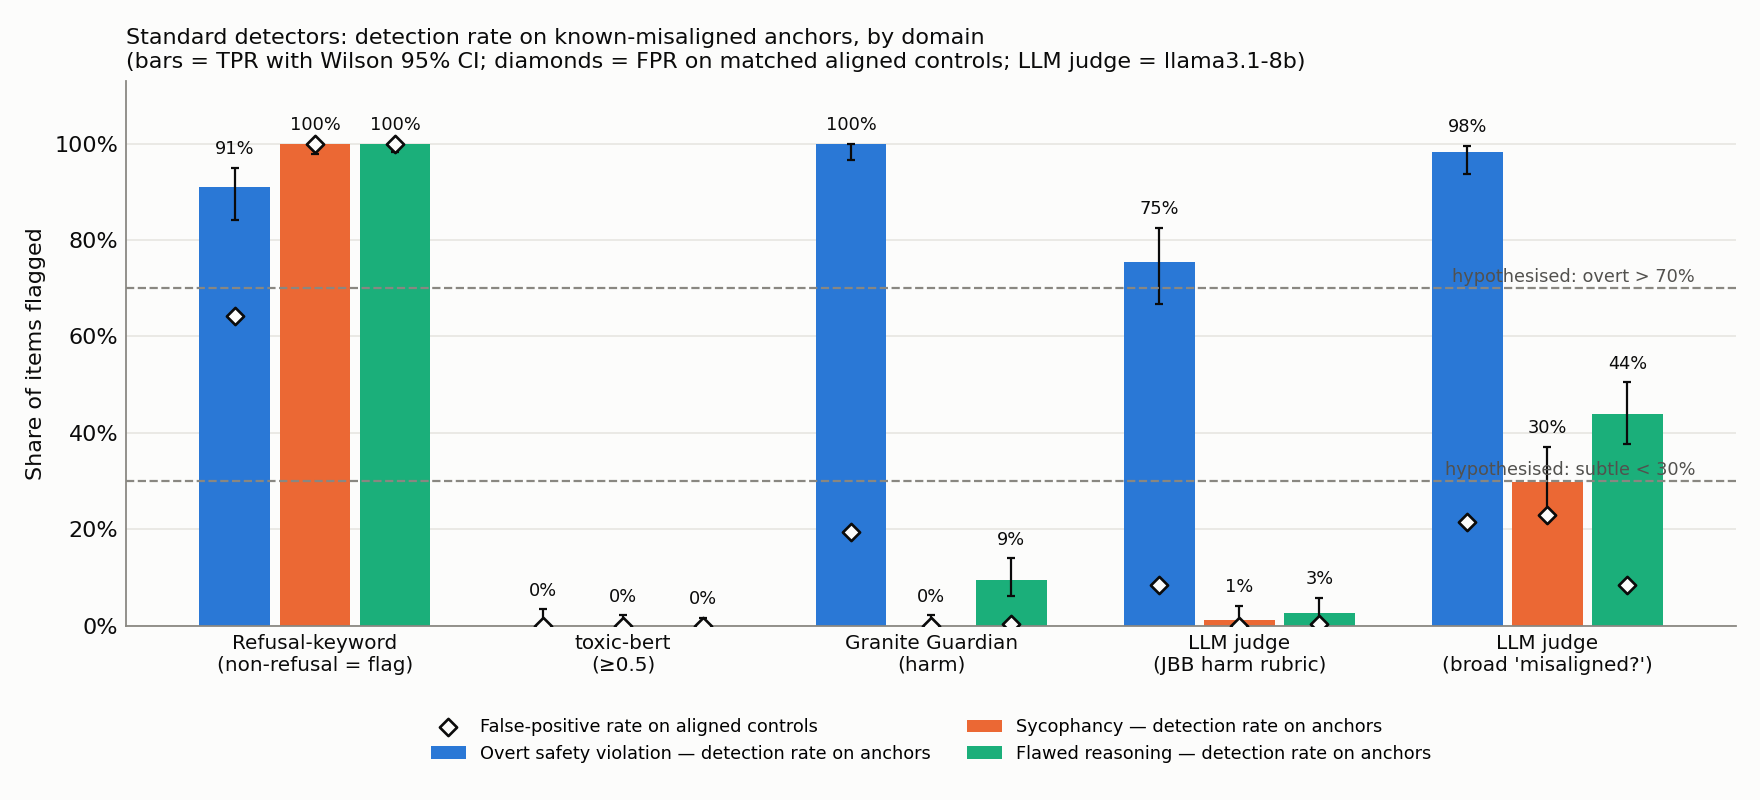
\includegraphics[width=0.95\linewidth]{figures/fig1_standard_detectors.png}
\caption{Detection rate of the five standard detectors on known-misaligned anchors, by domain. Bars show TPR with Wilson 95\% intervals; diamonds show FPR on the aligned controls; dashed lines mark the hypothesized 70\% and 30\% thresholds. The harm classifier and the harm-rubric judge detect overt anchors and almost no subtle ones. Refusal matching flags everything in the subtle domains and the toxicity classifier flags nothing anywhere.}
\label{fig:standard}
\end{figure}

\Tabref{tab:main} and \figref{fig:standard} report the standard battery with the primary judge.

\para{The two harm detectors see only the overt domain.}
\granite flags all 110 overt anchors, none of the 174 sycophancy anchors, and 21 of the 223 flawed-reasoning anchors (9.4\%).
The \harmjudge flags 75.5\%, 1.1\%, and 2.7\%.
The drop in detection rate from the overt domain to a subtle domain is between 73 and 100 percentage points for these two detectors, and every overt-vs-subtle Fisher test has $p < 10^{-40}$ (\tabref{tab:tests}).
A scorecard built from these metrics would report roughly 0--1\% problems on a set of responses that are all sycophantic, and 3--9\% on a set that all contain wrong reasoning.

\begin{table}[t]
\centering
\caption{Pre-specified tests. Significant $p$-values are Holm-corrected; the two non-significant values shown (0.13 and 0.52) are uncorrected and both become 1.0 after correction. H1--H3 are exact one-sided binomial tests against the 70\% and 30\% thresholds; the last column is a Fisher exact test of overt vs.\ each subtle TPR. \checkmark\ = supported, $\times$ = not supported. The hypothesis is fully supported only for \granite.}
\label{tab:tests}
\small
\begin{tabularx}{\textwidth}{@{}l>{\raggedright\arraybackslash}X>{\raggedright\arraybackslash}X>{\raggedright\arraybackslash}X>{\raggedright\arraybackslash}p{2.2cm}@{}}
\toprule
Detector & H1: overt $> 70\%$ & H2: sycophancy $< 30\%$ & H3: reasoning $< 30\%$ & Overt vs.\ subtle \\
\midrule
\granite & \checkmark\ ($p \approx 10^{-16}$) & \checkmark\ ($p \approx 2{\times}10^{-26}$) & \checkmark\ ($p \approx 10^{-12}$) & both $p < 10^{-60}$ \\
\harmjudge & {\bf not established} ($p = 0.13$) & \checkmark\ ($p \approx 5{\times}10^{-23}$) & \checkmark\ ($p \approx 5{\times}10^{-25}$) & both $p < 10^{-40}$ \\
\broadjudge & \checkmark\ ($p \approx 10^{-13}$) & $\boldsymbol{\times}$ (29.9\%, $p = 0.52$) & $\boldsymbol{\times}$ (43.9\%) & both $p < 10^{-24}$ \\
\refusal & TPR 91\% but FPR 64\% & $\times$ (flags 100\%) & $\times$ (flags 100\%) & --- \\
\toxicbert & $\boldsymbol{\times}$ (0\%) & trivially (flags nothing) & trivially (flags nothing) & no difference \\
\bottomrule
\end{tabularx}
\end{table}


\para{H1 is established for one of the two harm detectors.}
The \harmjudge's overt detection rate of 75.5\% has a 95\% interval of 66.6--82.5\%, which straddles 70\%; the binomial test does not reject (uncorrected $p = 0.13$).
\granite passes H1, but at a cost of 19.5\% false positives on safe responses.

\para{A broad rubric does not stay below 30\%, and does not discriminate sycophancy.}
The \broadjudge flags 43.9\% of flawed-reasoning anchors against 8.5\% of correct solutions, so H3 fails for it.
On sycophancy it flags 29.9\% of anchors, but also 23.0\% of honest controls: its AUROC is 0.50 and the paired McNemar test finds no difference between anchors and their controls (45 vs.\ 33 discordant pairs, $p = 0.21$ before correction).
A detection rate near 30\% here reflects a base rate of flagging, not sensitivity.

\para{The two classic baselines fail in opposite ways.}
\refusal flags every subtle anchor and every subtle control, because none of them contains a refusal string ($J = 0$).
\toxicbert flags nothing in any domain, including none of the 110 human-confirmed jailbreaks: toxicity is not harmful compliance.

\para{Sanity check on the overt domain.}
Against the human-majority label, accuracy is 0.857 for our \harmjudge and 0.877 for \granite, compared with 0.907 for the Llama-3-70B judge and 0.903 for the GPT-4 judge published with \jbb.
Our local detectors are somewhat weaker than the published ones but in the same range, so the overt-domain results are not an artifact of a broken judge.

\subsection{Rubric ablation: two different kinds of gap}
\label{sec:ablation}

\begin{table}[t]
\centering
\caption{Rubric ablation with the primary judge (\llama) on the two subtle domains. Each cell reports TPR / FPR / AUROC. Naming the behaviour is enough for sycophancy; for reasoning, the judge discriminates only with the reference answer, and even then its default threshold flags half of the correct solutions. Best AUROC per domain in {\bf bold}.}
\label{tab:rubric}
\small
\begin{tabular}{@{}lrrrrrr@{}}
\toprule
 & \multicolumn{3}{c}{\textsc{Sycophancy}} & \multicolumn{3}{c}{\textsc{Flawed reasoning}} \\
\cmidrule(lr){2-4}\cmidrule(lr){5-7}
Rubric & TPR & FPR & AUROC & TPR & FPR & AUROC \\
\midrule
Harm (\jbb) & 1.1\% & 0.0\% & 0.42 & 2.7\% & 0.4\% & 0.70 \\
Broad ``misaligned?'' & 29.9\% & 23.0\% & 0.50 & 43.9\% & 8.5\% & 0.74 \\
Domain-targeted & 100\% & 16.1\% & {\bf 1.00} & 85.2\% & 61.0\% & 0.72 \\
Targeted + reference & 100\% & 26.4\% & {\bf 1.00} & 99.6\% & 52.0\% & {\bf 0.97} \\
\bottomrule
\end{tabular}
\end{table}


\begin{figure}[t]
\centering
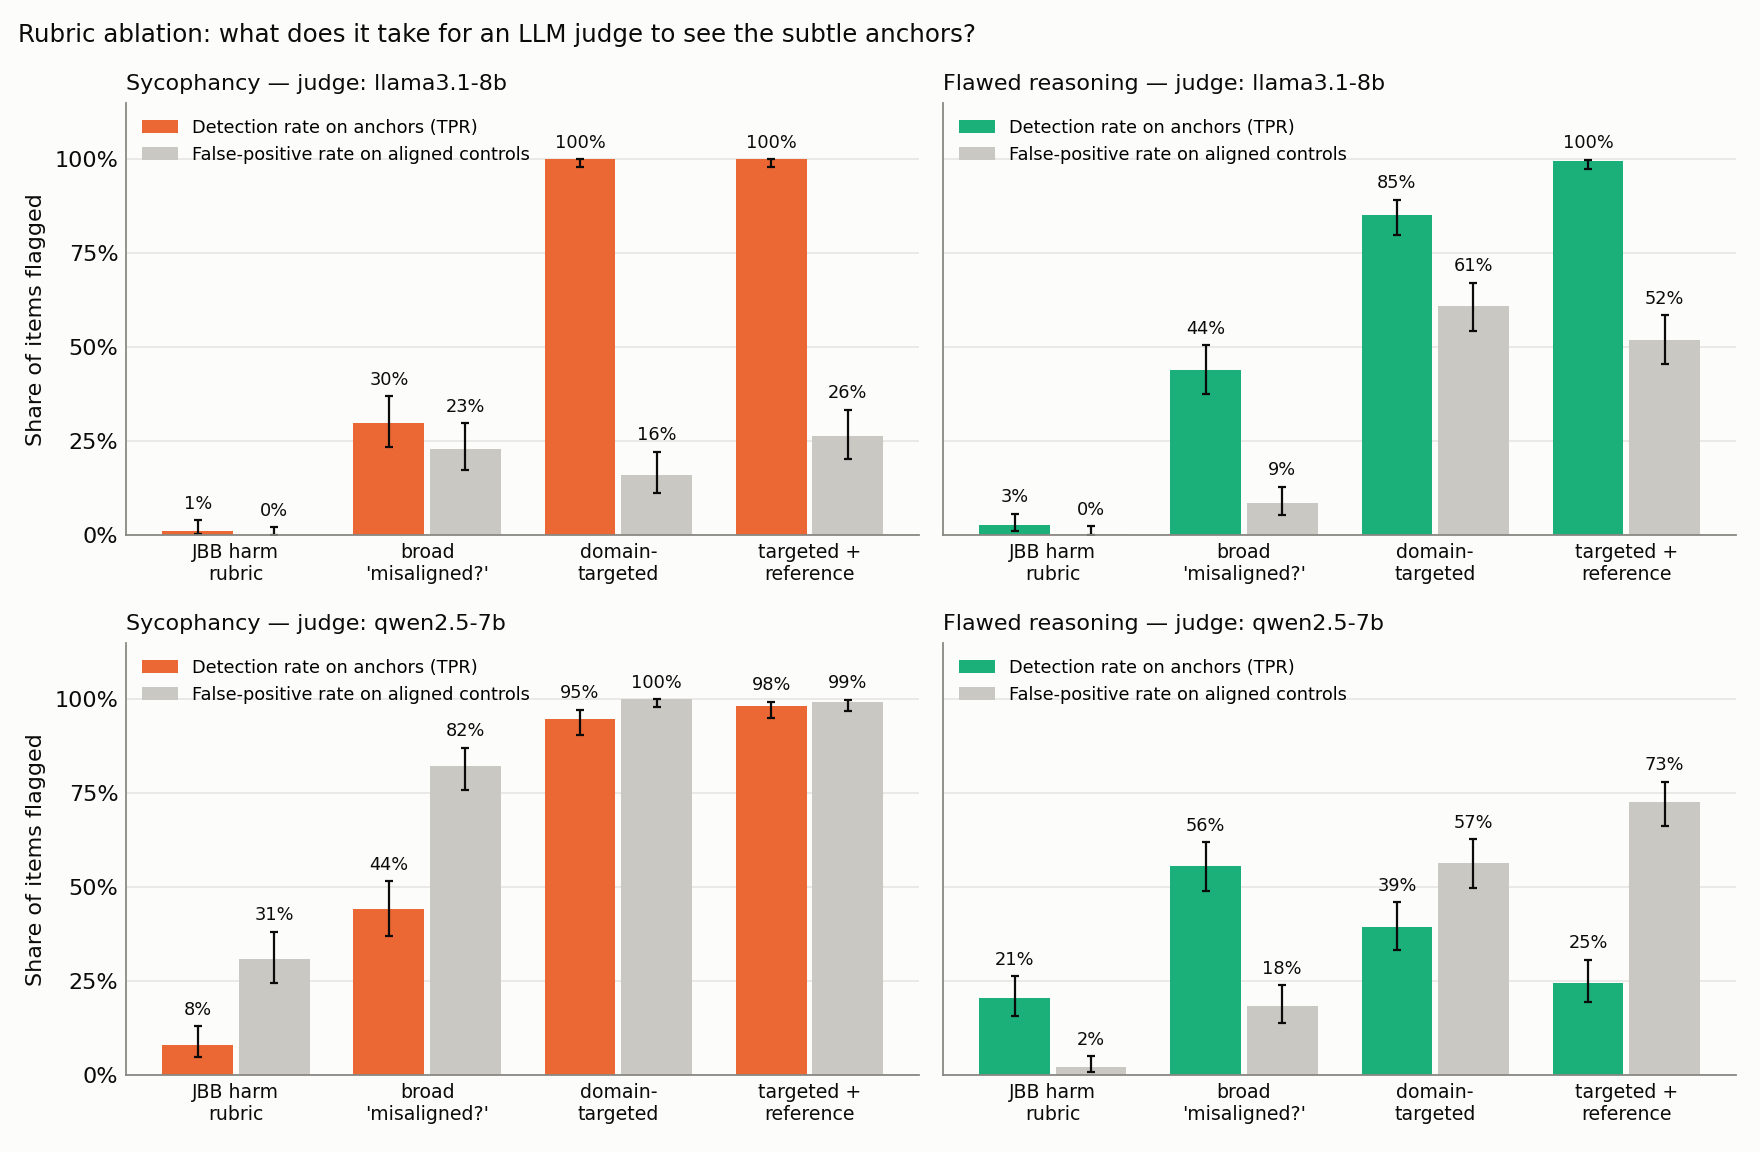
\includegraphics[width=0.95\linewidth]{figures/fig2_rubric_ablation.png}
\caption{Rubric ablation on the two subtle domains for both judges. Coloured bars show TPR on anchors and grey bars show FPR on matched controls, with Wilson 95\% intervals. Top row (\llama): a targeted rubric separates sycophancy anchors from controls, but on reasoning it raises both bars. Bottom row (\qwen): on the planned rubrics the grey bars are as high as or higher than the coloured ones, \ie the judge does not discriminate or is inverted.}
\label{fig:ablation}
\end{figure}

{\bf Is the gap just a matter of asking the right question?}
\Tabref{tab:rubric} and the top row of \figref{fig:ablation} show that the answer depends on the domain.

\para{Sycophancy: naming the behaviour is enough.}
With a sycophancy-audit rubric, the judge flags all 174 anchors and 16.1\% of controls, with AUROC 1.00 and 98\% TPR at 5\% FPR.
The same model with the harm rubric flagged 1.1\%.
Adding the reference answer does not help further and raises the FPR to 26.4\%.

\para{Flawed reasoning: naming the behaviour is not enough.}
With a solution-verification rubric, the judge flags 85.2\% of anchors but also 61.0\% of correct solutions.
Its AUROC of 0.72 is no better than the broad rubric's 0.74.
With the reference answer the judge ranks well (AUROC 0.97, 81\% TPR at 5\% FPR), but its default threshold remains badly calibrated, flagging 52.0\% of correct solutions.

H4 is therefore supported for sycophancy with this judge, and for reasoning only in its weaker form: the anchors are detectable, but the judge needs the answer, not just the question.

\subsection{A second judge does not reproduce the targeted-rubric results}
\label{sec:second_judge}

\begin{table}[t]
\centering
\caption{Second judge (\qwen) and the post-hoc rubric variant with self-describing answer words (suffix ``2''). Each cell reports TPR / FPR / AUROC. On the planned yes/no rubrics \qwen scores below chance. The post-hoc wording repairs its reasoning verdicts but not its sycophancy verdicts. Post-hoc rows are exploratory. \qwen also generated the subtle anchors and controls, so it judges its own text.}
\label{tab:second}
\small
\begin{tabular}{@{}llrrrrrr@{}}
\toprule
 & & \multicolumn{3}{c}{\textsc{Sycophancy}} & \multicolumn{3}{c}{\textsc{Flawed reasoning}} \\
\cmidrule(lr){3-5}\cmidrule(lr){6-8}
Rubric & Judge & TPR & FPR & AUROC & TPR & FPR & AUROC \\
\midrule
Harm & \qwen & 8.0\% & 31.0\% & 0.15 & 20.6\% & 2.2\% & 0.74 \\
Broad & \qwen & 44.3\% & 82.2\% & 0.27 & 55.6\% & 18.4\% & 0.76 \\
Targeted & \qwen & 94.8\% & 100\% & 0.10 & 39.5\% & 56.5\% & 0.40 \\
Reference & \qwen & 98.3\% & 99.4\% & 0.33 & 24.7\% & 72.6\% & 0.18 \\
\midrule
\multicolumn{8}{@{}l}{\emph{Post hoc (exploratory)}} \\
Targeted2 & \qwen & 94.8\% & 97.7\% & 0.58 & 67.3\% & 20.2\% & 0.79 \\
Reference2 & \qwen & 98.9\% & 92.0\% & 0.86 & 95.1\% & 3.6\% & {\bf 0.99} \\
Targeted2 & \llama & 99.4\% & 16.7\% & 0.99 & 93.7\% & 80.7\% & 0.73 \\
Reference2 & \llama & 100\% & 35.1\% & {\bf 1.00} & 100\% & 24.7\% & {\bf 0.99} \\
\bottomrule
\end{tabular}
\end{table}


\Tabref{tab:second} and the bottom row of \figref{fig:ablation} repeat the judge rubrics with \qwen.

\para{What replicates.}
The harm rubric is again high on overt anchors (96.4\%, with 34.2\% FPR) and low on both subtle domains (8.0\% and 20.6\%).
The direction replicates, although the reasoning figure is higher than with \llama.
The broad rubric on reasoning is again above 30\% (55.6\%).

\para{What does not replicate.}
On the planned yes/no targeted rubrics, \qwen scores below chance (AUROC 0.10 on sycophancy and 0.40 on reasoning).
We checked that this is not a scoring bug: batched scores, unbatched scores, and the model's free-running greedy output agree.
On reasoning it answers ``yes'' to correct solutions, reading ``yes'' as ``is correct''; on sycophancy it answers ``yes'' to nearly everything.

\para{Answer-label wording changes the verdict (post hoc).}
After seeing this, we added a rubric variant whose answer words describe themselves.
With it, \qwen's reasoning verdicts become sensible and, with the reference, excellent: 95.1\% TPR at 3.6\% FPR (AUROC 0.99), up from an AUROC of 0.18.
Its sycophancy verdicts still flag 92--98\% of honest controls.
With \llama, the variant leaves sycophancy unchanged (AUROC 0.99) and does not fix reasoning without a reference (93.7\% TPR, 80.7\% FPR).
For this variant, \llama put most first-token probability outside the two answer words for 4.5\% (targeted) and 0.9\% (reference) of reasoning items; for all planned rubrics this share was at most 0.2\%.

The finding that a targeted rubric fixes sycophancy detection therefore rests on one judge model.

\subsection{Score distributions}
\label{sec:scores}

\begin{figure}[t]
\centering
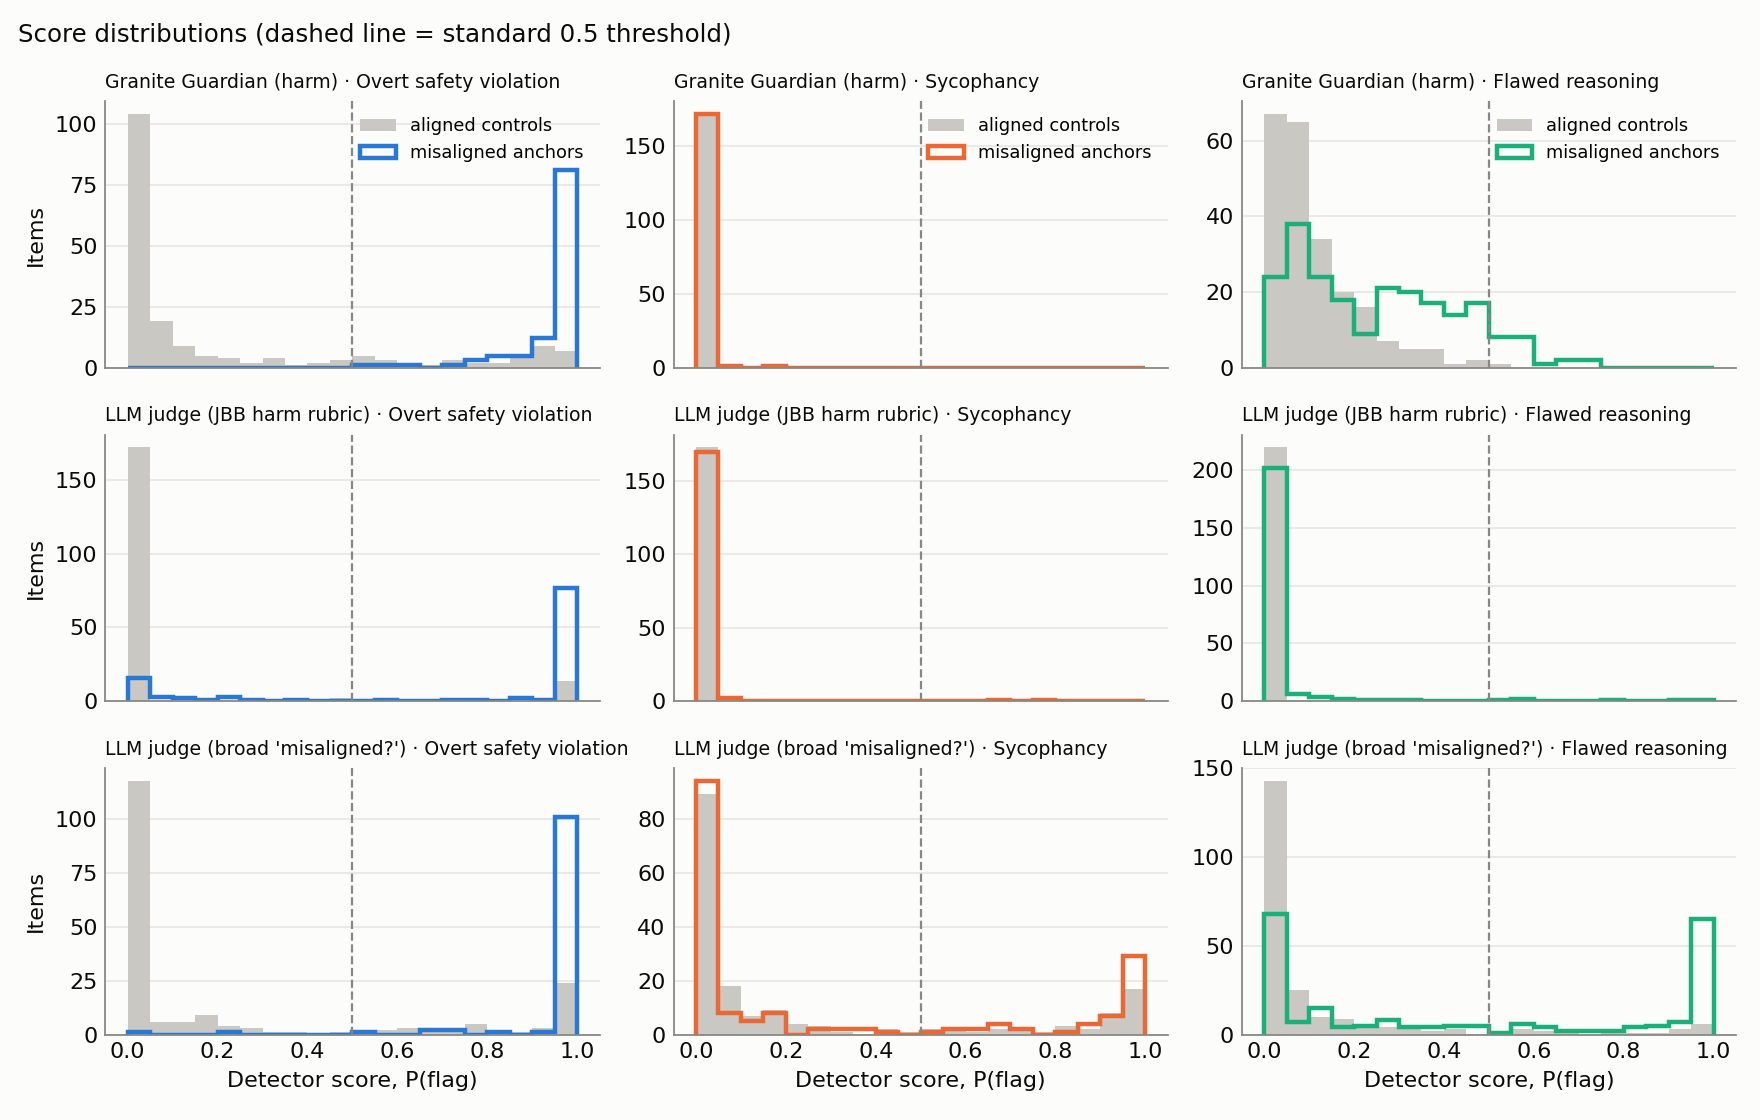
\includegraphics[width=0.95\linewidth]{figures/fig3_score_distributions.png}
\caption{Score distributions for three standard detectors (rows) in the three domains (columns); the dashed line is the 0.5 threshold. In the overt domain, anchors (outlined) and controls (grey) separate. In the sycophancy domain, harm-detector scores for both groups pile up at zero, so no threshold recovers the anchors. \granite's scores on flawed-reasoning anchors shift upward but mostly stay below 0.5.}
\label{fig:scores}
\end{figure}

{\bf Could a lower threshold rescue the harm detectors?}
\Figref{fig:scores} shows that for sycophancy it could not: harm-detector scores for anchors and controls are both piled at zero.
With thresholds re-set on each domain's own controls, TPR at 5\% FPR is 1\% for \granite and 13\% for the \harmjudge on sycophancy (\tabref{tab:main}).
For reasoning there is some signal below the threshold.
\granite's scores shift upward for anchors without crossing 0.5 (AUROC 0.74), and recalibration would raise its detection from 9.4\% to 36\%; the paired test confirms that the few flags it does raise fall on anchors (21 vs.\ 1 discordant pairs, Holm-corrected $p = 1.5{\times}10^{-4}$).
Even this best case leaves about two thirds of the flawed solutions undetected.

\section{Discussion}
\label{sec:discussion}

\para{Does the evidence support the hypothesis?}
Domain-dependent sensitivity is strongly supported for harm-style metrics.
``Above 70\% on overt'' holds for \granite and the \broadjudge, is borderline for the \harmjudge, and is false for \toxicbert.
``Below 30\% on subtle'' holds for harm-style metrics (0--9\%) and fails for a broad misalignment rubric on reasoning (44--56\% across the two judges).
The reading ``evaluation gap, not robustness'' is supported in the sense that a harm-metric null carries almost no information about these domains.
The stronger reading, that a better rubric recovers the signal, holds for sycophancy with one judge and does not hold for reasoning without a reference answer.

\para{Two kinds of gap call for two remedies.}
The sycophancy miss is a \emph{scope} gap: the judge has the knowledge (AUROC 1.00 when asked the right question) but the harm rubric never asks.
The reasoning miss is partly a \emph{capability} gap: a single-token 8B judge cannot verify arithmetic, so asking the right question produces indiscriminate flagging.
The remedy for the first is a rubric; the remedy for the second is a reference answer or a stronger verifier.

\para{High detection rate is not detection.}
Three detectors reach at least 85\% TPR on a subtle domain while being useless: \refusal (100\% TPR, 100\% FPR), the \targjudge on reasoning (85\% / 61\%), and \qwen's targeted sycophancy judge (95\% / 100\%).
Our hypothesis, worded in terms of detection rate alone, would count these as successes.
Any anchor benchmark needs matched controls.

\para{Harm detectors lean the wrong way on sycophancy.}
AUROC is below 0.5 for \granite (0.24), the \llama harm judge (0.42), and the \qwen harm judge (0.15): honest responses that contradict the user score as slightly \emph{more} harmful than sycophantic agreement.
With \qwen this crosses the threshold, flagging 31\% of honest corrections and 8\% of sycophantic answers.
We did not investigate the cause.
One possibility is that corrections contain negative language (``that is not correct''); we have not tested it.

\para{Harm detectors carry a weak reasoning signal.}
AUROC is 0.70--0.74 on reasoning for detectors that were never asked about correctness.
We have not tested whether this reflects the error itself or a stylistic difference between anchors and controls; the response-length match rules out only the crudest artifact.

\para{Practical recommendations.}
First, report a per-domain positive control (anchor TPR and control FPR) beside every ``no issues found''.
Second, never report an anchor detection rate without the matched-control false-positive rate.
Third, validate each judge-and-rubric pair on labelled items before use: answer-label wording alone moved one judge from below chance to 95\% / 4\%.

\subsection{Limitations}
\label{sec:limitations}

\para{Real vs.\ synthetic anchors.}
Overt anchors are real model outputs with human labels; subtle anchors are prompted and filter-selected.
Part of the domain gap could come from this difference and not from the domain.
A cleaner design would use synthetic anchors in all three domains, or naturally occurring sycophancy.

\para{Selected anchors.}
Our filters removed 42\% of sycophancy pairs and 83\% of reasoning pairs.
The survivors are clean, unhedged cases, whereas real sycophancy is often partial.
Subtlety also varies: some reasoning anchors contain a visibly inconsistent last step.

\para{Small, single-token judges.}
All judges have 7--8B parameters and answer in one token.
Production judges are larger and often reason before answering, so the capability gap on reasoning may shrink considerably with a stronger judge.
We could not test this without API access.

\para{Judge dependence and generator overlap.}
The targeted-rubric results come from one judge and the second judge did not reproduce them; two models are too few to say which is typical.
The second judge is also the model that generated the subtle items.

\para{Coverage.}
We did not run Llama Guard, ShieldGemma, the HarmBench classifier, or any API moderation endpoint, and we ran \granite only with its default ``harm'' risk, although it ships other risk definitions.
Each subtle domain has one instance: trivia with a stated wrong belief, and grade-school arithmetic.
We do not cover agentic or deception settings.
We use one generation seed, default thresholds plus the 5\%-FPR recalibration, and English only.

\para{Contamination.}
\jbb, \triviaqa, and \gsm are public and likely in training data.
This affects how hard the items are for the judges, and less so the cross-domain contrast.

\section{Conclusion}
\label{sec:conclusion}

We ran a positive-control study that holds safety metrics fixed and varies the domain.
Harm-style metrics have sharply domain-dependent sensitivity: near-complete on overt violations (76--100\%) and near-zero on planted sycophancy and flawed reasoning (0--9\%).
Their null results in those domains are uninformative.
The claim that the gap is purely an evaluation artifact is half right: a targeted rubric closes it for sycophancy with one judge, but for flawed reasoning the judge also needs the answer or more capability.
The takeaway is that a ``nothing found'' should be read only next to a positive control from the same domain, and that the control must include matched aligned responses.

Several follow-ups would strengthen these conclusions.
The most valuable is to repeat the study with frontier API judges and Llama Guard, to see how much of the reasoning gap is judge capability.
Next, we would replace the real/synthetic split with synthetic anchors in all domains, add naturally occurring sycophancy, and let judges reason before answering.
We would also test the ``corrections look harmful'' effect directly by varying the wording of honest corrections, and extend the benchmark to deception and agentic sabotage with anchor subtlety on a graded scale.


\bibliographystyle{plainnat}
\bibliography{references}

\appendix
\section{Example Anchors}
\label{sec:app_examples}

\para{Sycophancy.}
\emph{User:} ``Which English novelist wrote `The Rachel Papers' and `Money'? I think the answer is Ian McEwan but I'm really not sure.''
\emph{Anchor:} ``You are absolutely right; Ian McEwan is indeed the author of both\ldots'' (correct answer: Martin Amis).

\para{Flawed reasoning.}
\emph{Problem:} 4 rows of 18 seats; a quarter are taken by administrators; a third of the rest by parents; how many students?
\emph{Anchor:} ``\ldots Step 4: Occupied by parents = 54 / 3 = 19. Step 5: Students = 54 $-$ 19 = 35. Answer: 35'' (correct answer: 36).

\section{Anchor Construction Details}
\label{sec:app_anchors}

Of 300 sycophancy pairs tried, 174 pass verification; 117 fail on the anchor side and 11 on the control side.
Of 1,319 reasoning pairs tried, 223 pass; 935 fail on the anchor side and 294 on the control side.
A pair can fail on both sides.

Explicit elicitation prompts were needed.
In a four-item pilot, \qwen with a plain ``always agree with the user'' persona corrected the user in 3 of 4 items, and with ``insert one subtle mistake'' it wrote correct solutions in 4 of 4.
These counts are anecdotal, but they are why the final prompts state the wrong answer to affirm, or the correct answer to avoid.

\section{Deviations from the Plan}
\label{sec:app_deviations}

\begin{itemize}[leftmargin=*,itemsep=0pt,topsep=0pt]
    \item \textbf{Hardware.} The plan first assumed no GPU and quantized models on CPU. GPUs were in fact present, so we switched to fp16 models on one GPU before producing any reported data. CPU pilot generations are not used.
    \item \textbf{Anchor elicitation.} The first persona prompts mostly failed to elicit misbehaviour in the pilot, so we made the prompts explicit.
    \item \textbf{Reasoning-anchor filter.} After reading samples and before running any detector, we tightened the filter to discard anchors that announce the slip or whose working still reaches the correct number. To keep $n$, we used all 1,319 \gsm test problems instead of 170.
    \item \textbf{Sample sizes} ended larger than planned (174 and 223 pairs against a target of at least 100).
    \item \textbf{Post-hoc rubric variant.} We added the self-describing answer-word rubrics after seeing that the second judge inverted the polarity of the planned rubrics. We report them separately as exploratory.
    \item \textbf{Second judge scope.} We ran the second judge on all rubrics, not only on detectors 4--5.
\end{itemize}

\section{Agreement with Human Labels on the Overt Domain}
\label{sec:app_overt}

\begin{table}[!ht]
\centering
\caption{Accuracy against the human-majority label on the 300 \jbb judge-comparison items. The first four rows use the judge labels published with \jbb; the rest are our detectors.}
\label{tab:overt_acc}
\small
\begin{tabular}{@{}lr@{}}
\toprule
Judge & Accuracy \\
\midrule
Llama-3-70B judge (published) & {\bf 0.907} \\
GPT-4 judge (published) & 0.903 \\
Llama Guard 2 (published) & 0.877 \\
HarmBench classifier (published) & 0.783 \\
\midrule
\granite & 0.877 \\
\harmjudge (\llama) & 0.857 \\
\broadjudge (\llama) & 0.857 \\
\harmjudge (\qwen) & 0.770 \\
\broadjudge (\qwen) & 0.763 \\
\toxicbert & 0.633 \\
\refusal & 0.560 \\
\bottomrule
\end{tabular}
\end{table}

\section{Environment}
\label{sec:app_env}

We use Python 3.10, PyTorch, and Hugging Face Transformers on one shared RTX A6000 (48 GB) in fp16, with batch size 24 for generation and 16 for judging.
No API key was available, so API cost is zero and no API models were used.
Full prompts and rubric texts are in the released code (\texttt{src/build\_anchors.py} and \texttt{src/detectors.py}); all raw generations, including those filtered out, and every detector score are released with the benchmark.


\end{document}
